%-----------------------------------------------------------------------------
%	 Diseño e Implementación
%-----------------------------------------------------------------------------

\lhead[\thepage]{Diseño e Implementación \thechapter. \rightmark}
\rhead[Diseño e Implementación \thechapter.1 \leftmark]{\thepage}

%	Capitulo 6: Diseño e Implementación
\chapter{Diseño e Implementación}
\markboth{Diseño e Implementación}{Diseño e Implementación}
En este capitulo se presenta a partir del problema planteado una solución basada en una aplicación web que es capaz de poder tomar los datos de dispositivos IoT entre sensores y actuadores con los que interactuar, a través de la integración de diversas herramientas de visualización y control, incluyendo la posibilidad tanto de presentar indicadores de datos en tiempo real, así como también interactuar con data histórica para su análisis.\\

Todas las tecnologías aquí presentadas son software y hardware libre por lo que pueden ser adaptadas rápidamente según los requerimientos funcionales del problema y cumplen con legislativa local para poder ser exploradas a fondo. 

%	Sección uno: Diseño
\section{Diseño}
\lhead[\thepage]{\thesection. Diseño}
El diseño propuesto para examinar la solución al problema planteado pasa por dos etapas:
\begin{itemize}
\item Prototipos de uno o más dispositivos IoT que sean capaces de generar información real de su entorno, explorando los métodos más adecuados para poder llevar a cabo la tarea de transmitir información, así como explorar las posibilidades de procesamiento de cada dispositivo.
\item Aplicación web que incluya la posibilidad de visualizar los datos, monitorear y controlar los dispositivos IoT que se encuentren registrados. Para ello se integraran una serie de herramientas de software que aprovechen las mejores características de su diseño para poder cumplir con los objetivos planteados.
\end{itemize}

Dado que los dispositivos Raspberry Pi pueden usar un sistema operativo completo estos pueden operar de manera independiente a otros dispositivos, no siendo el caso del dispositivo Arduino Uno se complementa su integración haciendo uso de una computadora Apple iBook G4 para poder recibir y enviar la data de manera inalámbrica.\\

Siendo la idea examinar variables y comportamientos de dispositivos en un ambiente de un hogar inteligente junto con la variedad de placas programables, sensores y actuadores disponible se sugieren la creación de 4 prototipos de dispositivos IoT distintos:

\begin{itemize}
\item Un prototipo de dispositivo IoT usando Arduino Uno (junto al computador iBook G4) para representar un artefacto que se coloque en exteriores para obtener y representar variables ambientales y de recursos comunes en esas áreas. Para ello se destinan un sensor PIR HC-501, un sensor de test de nivel de agua Robodo Sen18, un sensor de temperatura DS1820, un led RGB para representar de manera visual la temperatura y una fotorresistencia LDR de 10K (véase figura: \ref{fig:arduino1}).
\begin{figure}[htb]
\centering
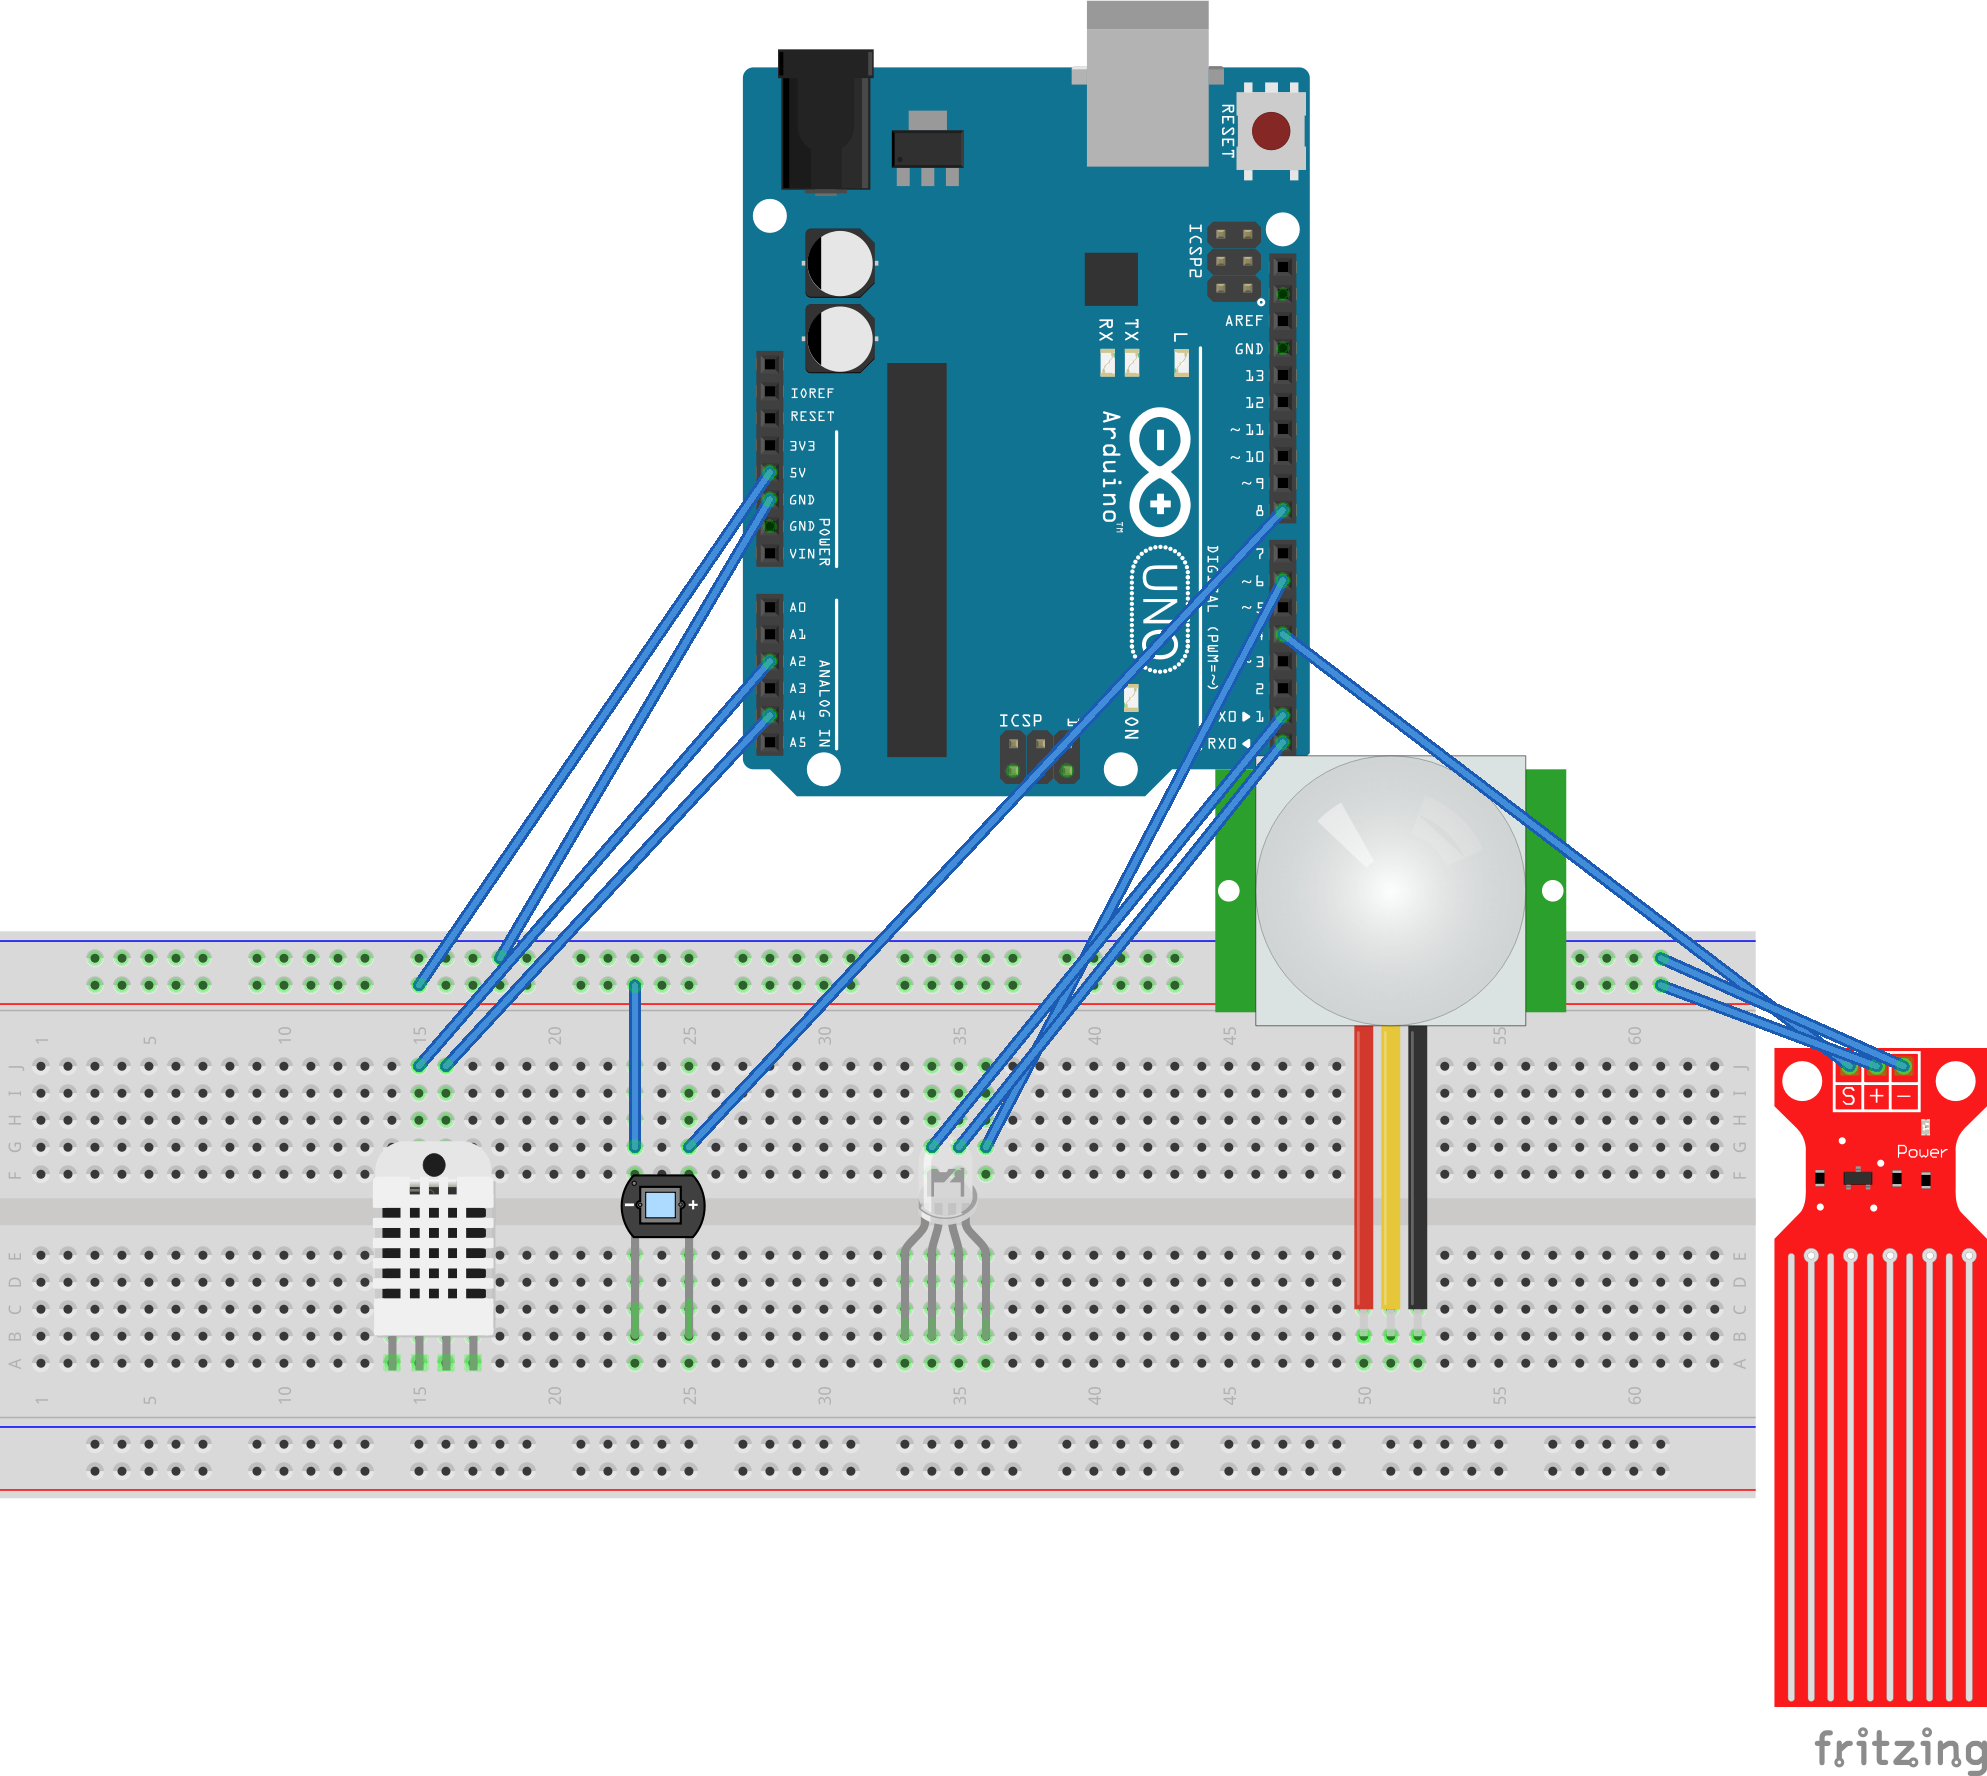
\includegraphics[scale=0.5]{./Figuras/arduino1.png}
\caption{Prototipo de dispositivo exterior usando Arduino Uno}
\label{fig:arduino1}
\vspace*{-10pt}
\end{figure}

\item Un prototipo de dispositivo IoT usando un Raspberry Pi 3 Modelo B para representar un artefacto que se coloca en un espacio interior para obtener y representar variables ambientales y recursos comunes en el área. Para ello se harán uso de un sensor de temperatura y humedad DHT11, un Led RGB para representar de manera visual la temperatura, un sensor de medición de distancia usando ultrasonido HC-SR504, un led rojo y un led verde operacionales para indicar presencia de movimiento con el sensor de movimiento, un un buzzer y un servomotor que dada una cierta distancia con el sensor de movimiento se accionaran y a su vez tocara una melodía, un conjunto de 3 leds blancos para representar bombillos en una habitación y por último un sensor de intensidad lumínica TSL2561 para medir la intensidad de la luz en la habitación.(véase figura: \ref{fig:rpi3javier}).
\begin{figure}[htb]
\centering
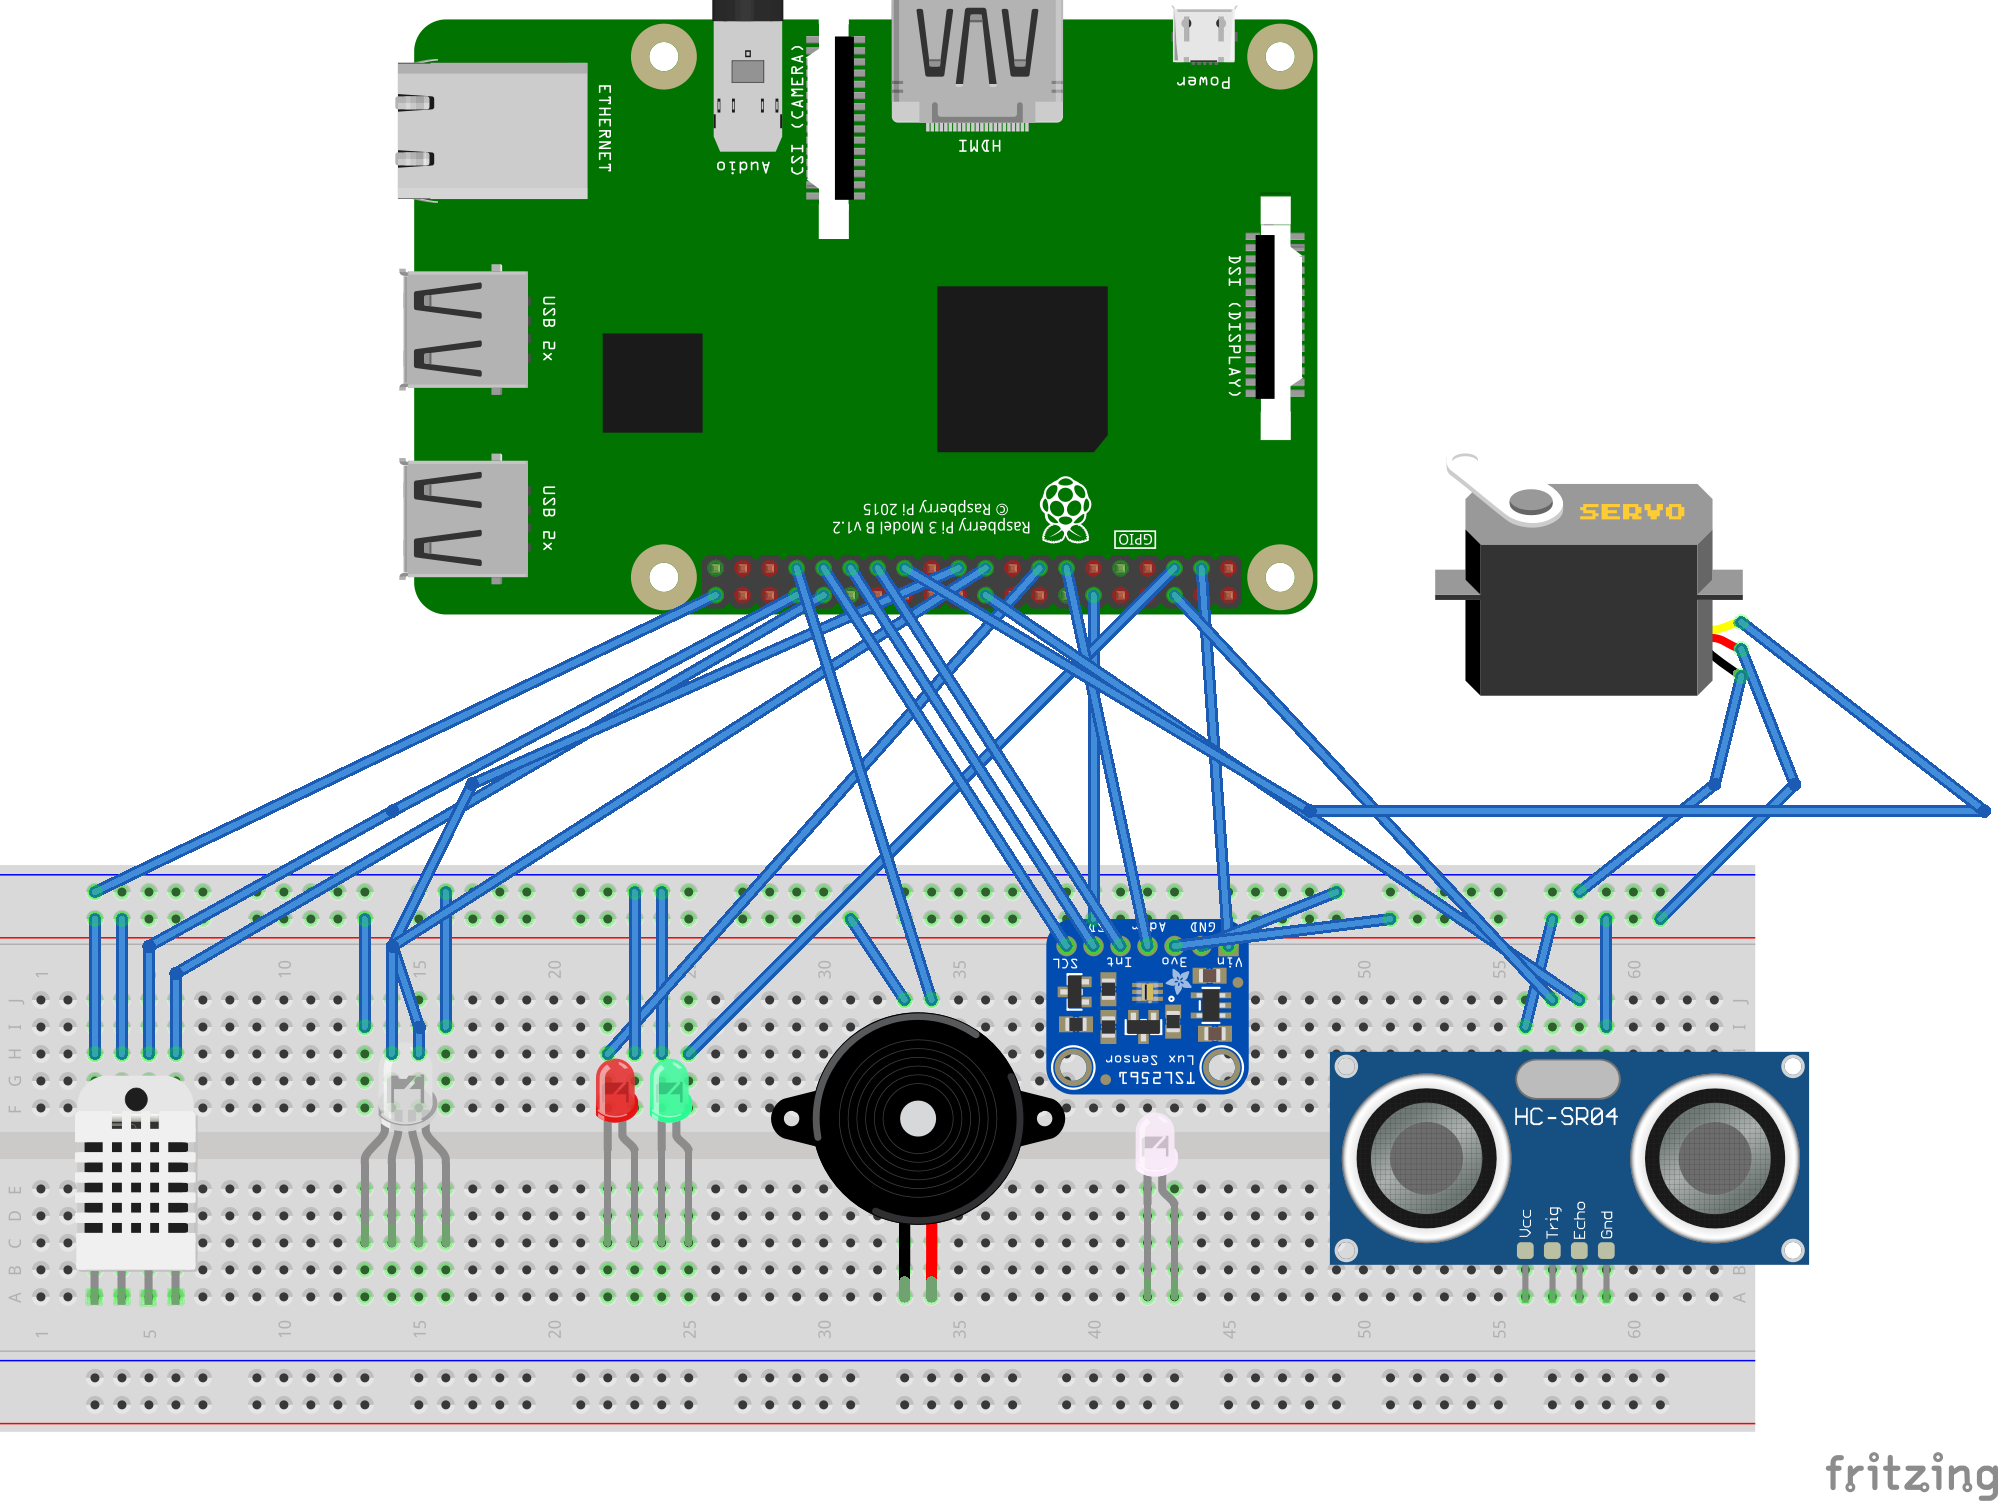
\includegraphics[scale=0.5]{./Figuras/rpi3javier.png}
\caption{Prototipo de dispositivo interior usando un Raspbery Pi 3 modelo B}
\label{fig:rpi3javier}
\vspace*{-10pt}
\end{figure}

\item Un prototipo de dispositivo IoT usando un Raspberry Pi zero para representar un artefacto pensado para en variables de seguridad y acceso que se coloca en un espacio interior. Para ello se harán uso de un lector RFID RC522, una pantalla LCD para representar la hora y darle la bienvenida al usuario, un led rojo y un led verde operacionales para indicar existencia de movimiento gracias a un sensor PIR HC-SR501, 3 leds blancos para representar bombillos (que se activen con movimiento).(véase figura:\ref{fig:rpizero_diagram}).
\begin{figure}[htb]
\centering
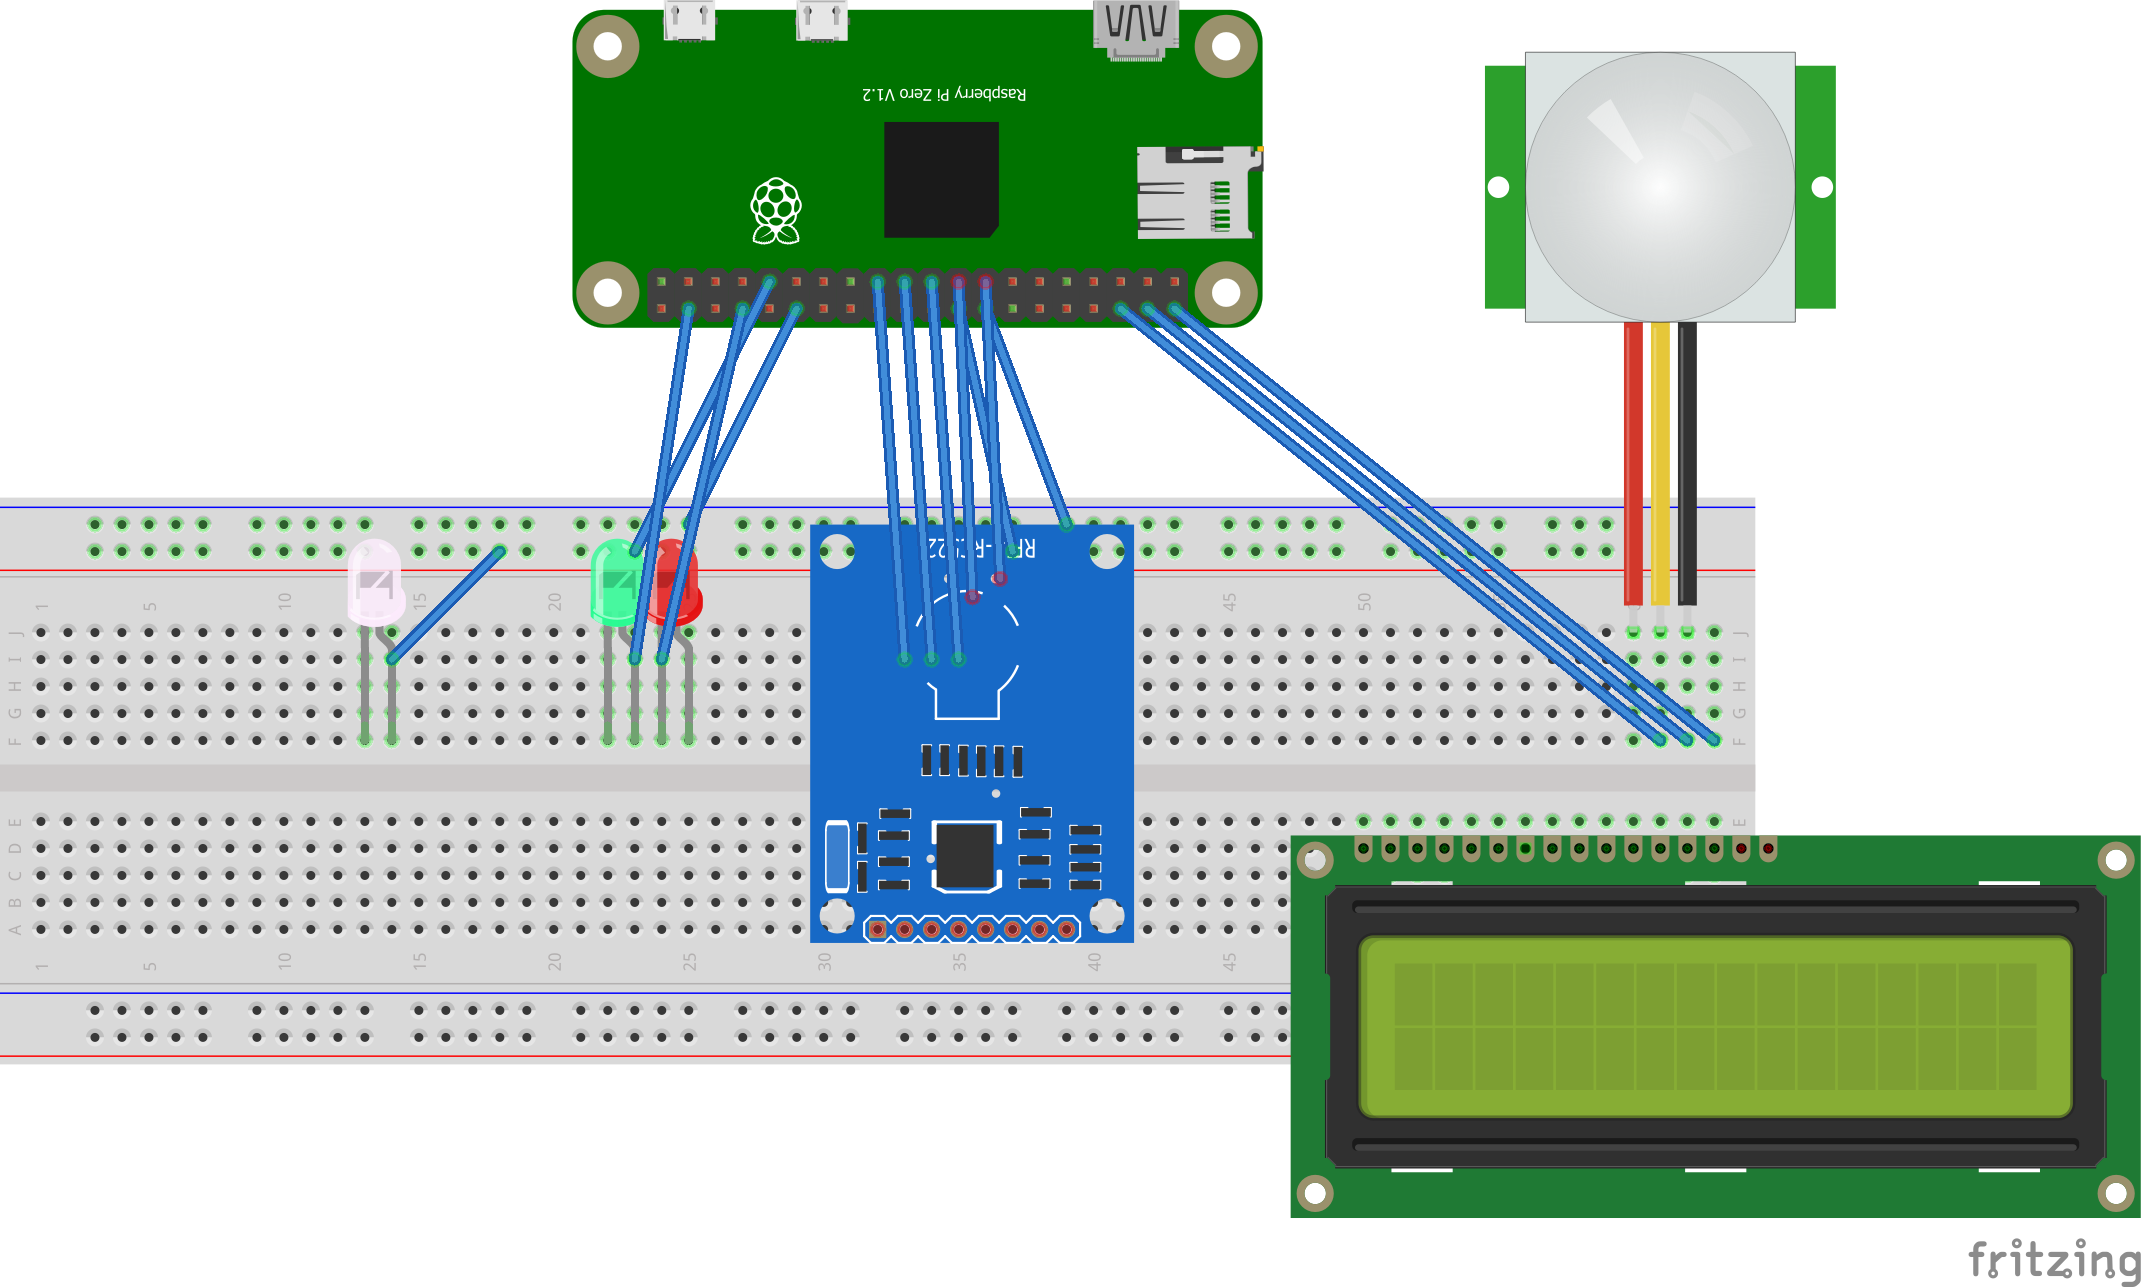
\includegraphics[scale=0.5]{./Figuras/rpizero_diagram.png}
\caption{Prototipo de dispositivo de seguridad usando un Raspbery Zero}
\label{fig:rpizero_diagram}
\vspace*{-10pt}
\end{figure}

\item Un prototipo de dispositivo IoT usando un Rapsberry Pi 3 Modelo B para representar una cámara inteligente capaz de detectar rostros de personas registradas y de desconocidos para alertar una posible intrusión usando un modelo de inteligencia artificial para ello. Se destina la cámara RaspiCam v1 para esta tarea.(véase figura:\ref{fig:rpipeter}). También dadas las capacidades computacionales de esta placa programable se establece que pueda usarse como punto de acceso para los otros prototipos y lugar de despliegue de la herramienta web para visualización, monitoreo y control de los prototipos. 
\begin{figure}[htb]
\centering
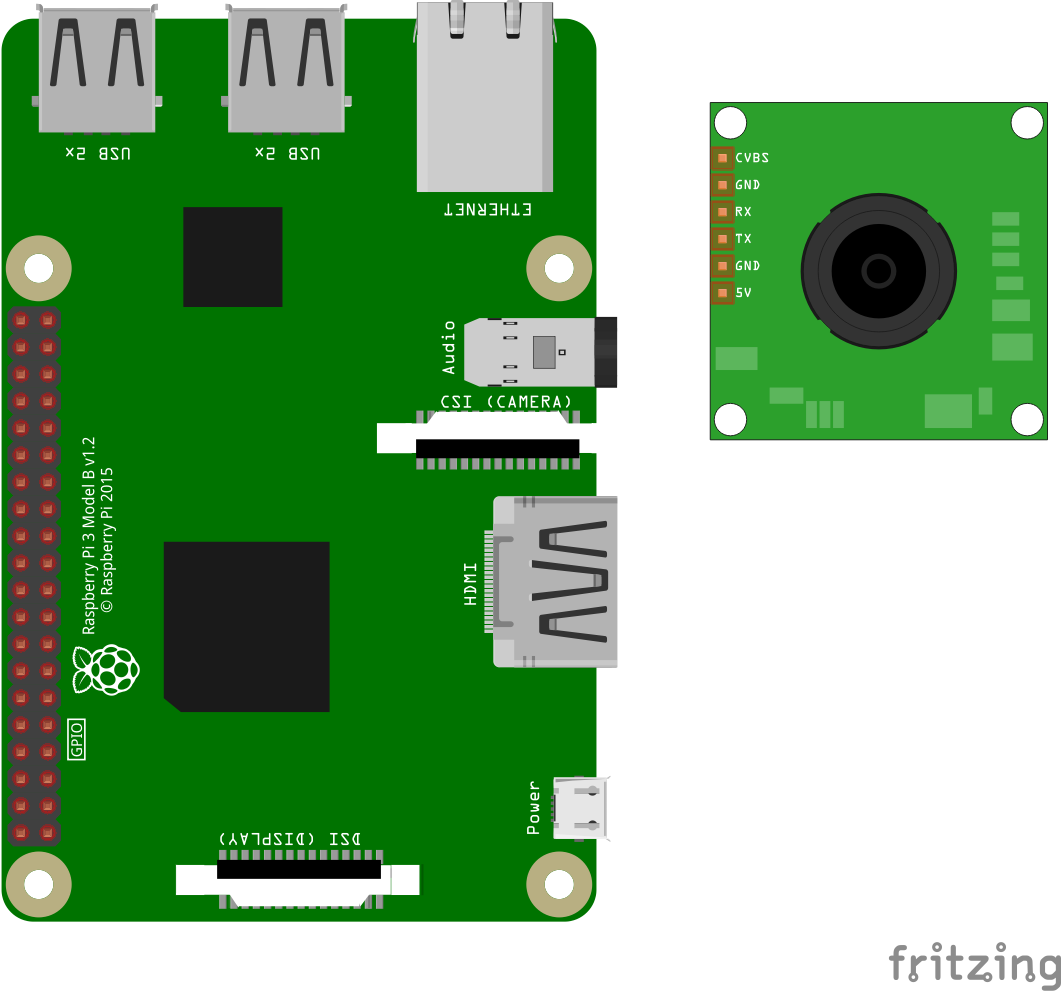
\includegraphics[scale=0.5]{./Figuras/rpipeter.png}
\caption{Prototipo de dispositivo de cámara de inteligente usando un Raspbery Pi 3 modelo B}
\label{fig:rpipeter}
\vspace*{-10pt}
\end{figure}

\end{itemize}

Con esta gama de distintos prototipos planteados para escenarios diferentes se hará obtención de data y generar acciones automáticas dependiendo del contexto que estos datos provean.  

\subsection{Software de Visualización, Monitoreo y Control}
La parte mas importante del planteamiento del problema se traduce en la falta de soluciones que permitan visualizar datos históricos y en tiempo real, junto con la capacidad de monitorear el estado de los dispositivos y la posibilidad final de controlarlos y establecer rutinas mas allá de su programación inicial.\\

Para ello y examinando las diversas opciones de tecnologías estudiadas e investigadas durante el marco teórico del seminario se propone la creación de un software que funcione de la siguiente manera: 
\begin{itemize}
\item Una infraestructura básica que permita conectar a los dispositivos de manera centralizada, capaz de funcionar usando protocolos y estándares existentes, a la vez que este diseñado para su utilización en dispositivos IoT. Basados en la investigación previa por sus ventajas, robustez y simplicidad de uso se opta por utilizar el protocolo MQTT\cite{iotprotocols} bajo la implementación Mosquitto\cite{ALight2017}.

\item Dada la naturaleza no estructurada de los datos enviados por los dispositivos IoT, se requiere una base de datos que pueda almacenar fácilmente dichos valores. Se tiene que tener en cuenta que esta base de datos debería estar orientada a la utilización de datos históricos y en tiempo real (dimensión de tiempo). Es por ello que basados en la investigación previa realizada y teniendo en cuenta la naturaleza de los datos y las tareas que se esperan del sistema manejador de base de datos, se toma la decisión de usar InfluxDB\cite{influxdb}, que es una base de datos orientada a series de tiempo con alta integración con otras herramientas disponibles en el mercado.

\item  Una herramienta web que sea capaz de desplegar la información de sensores, actuadores tanto de manera histórica como en tiempo real, además de gestionar y centralizar el control de dispositivos y rutinas extras, con la posibilidad de tener acceso a ella basado en registro de usuarios y que estos sean capaces de crear cuadros de mando adaptados a las necesidades de sus dispositivos y requerimientos. Esta parte de la propuesta busca no crear todo una suite desde 0 sino aprovechar herramientas ya existentes para ello. Teniendo en cuenta eso, se decide en primer lugar crear una webapp usando el lenguaje de programación Python\cite{whatspython} en su version 3 con el framework Django\cite{django} bajo una base de datos Postgresql\cite{postgresql} para almacenamientos de los datos referentes a esta aplicación. En cuanto al tema de visualización y monitoreo se establece el uso integrado de la aplicación web Grafana\cite{grafana} y del mismo modo, para el control de dispositivos y de flujos de trabajos se acepta finalmente el uso de la herramienta web Node-Red\cite{nodered}

\end{itemize}

Con estos componentes definidos y después de discutir sobre la mejor manera de desplegar este conjunto de tecnologías, buscando facilidad de operación y manutención así como la portabilidad y la independencia de plataformas se decide utilizar la mayor cantidad de componentes posibles como contenedores. Para ello el uso de docker\cite{docker}, comenzando por las integraciones y otros componentes esenciales (figura \ref{fig:componentes_hamaca}). Finalmente con estos componentes se establecen las siguientes directrices:

\begin{figure}[!htb]
\centering
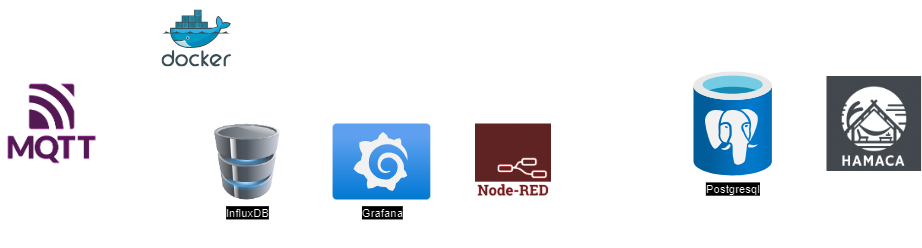
\includegraphics[scale=0.35]{./Figuras/componentes_hamaca.png}
\caption{Componentes sugeridos para la herramienta de visualización, monitoreo y control HAMACA}
\label{fig:componentes_hamaca}
\vspace*{-10pt}
\end{figure}


\begin{itemize}

\item Se usara Mosquitto como Broker MQTT para las comunicaciones entre los dispositivos y aquel elemento que lleve la información a la base de datos. Este estará centralizado en el mismo dispositivo donde se alojará la aplicación web, aunque se recalca el hecho que pueden existir multiples brokers bajo la arquitectura de MQTT, así como también que el broker puede ser configurado de manera externa.


\item La aplicación web HAMACA seguirá el paradigma cliente-servidor, con un front-end marcado y distinto a su back-end. La aplicación web solo dependerá de la base de datos PostgreSQL para almacenar variables de configuración, estadísticas de uso y aquellas que den soporte a la autenticación y gestión de usuarios.


\item La Base de datos InfluxDB solo ha de ser consultada por la integración a Grafana para la visualización y monitoreo óptimo de los datos haciendo uso de los dashboards configurables dentro de la aplicación. Grafana será embebido en la aplicación web HAMACA en su frontend. Al igual forma que la implementación de MQTT este puede existir en otro punto de red pero se sugiere el despliegue en el mismo dispositivo. 

\item La herramienta de control y de gestión de flujo de tareas automatizado Node-Red, al igual que Grafana será embebida sobre el frontend de la aplicación web HAMACA. Este componente podrá interactuar también con el broker MQTT para poder transmitir (y en algunos casos, también capturar directamente) los sensores y acturadores de los prototipos de dispositivos IoT.

\end{itemize}
De esta forma se presenta el diseño de la arquitectura de la solución para el problema de investigación como se puede notar en la figura \ref{fig:arquitectura_hamaca}
\begin{figure}[!htb]
\centering
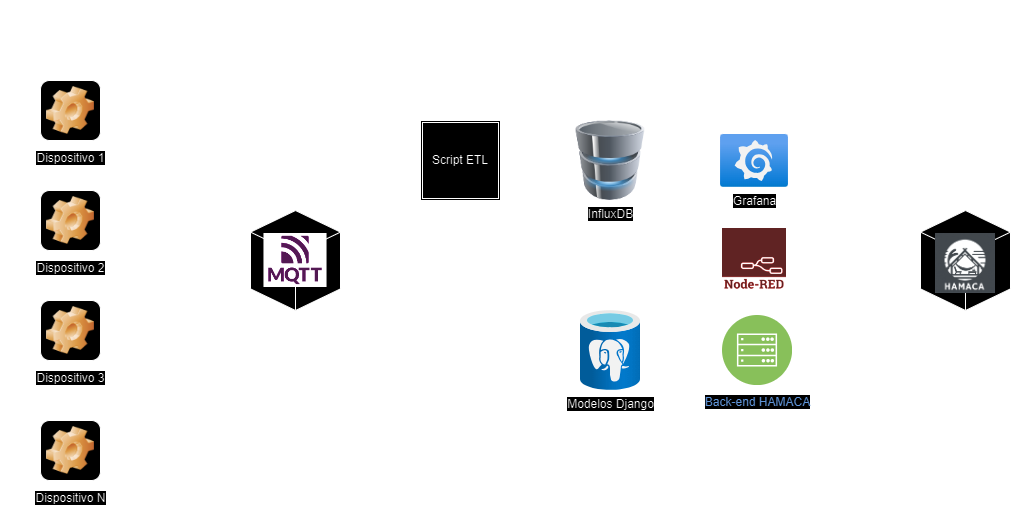
\includegraphics[scale=0.28]{./Figuras/arquitectura_hamaca.png}
\caption{Arquitectura de la solución propuesta}
\label{fig:arquitectura_hamaca}
\vspace*{-10pt}
\end{figure}

%	Sección dos: Implementación  de la solución 
\section{Implementación de la solución}
\lhead[\thepage]{\thesection. Implementación de la solución}
Siguiendo lo convenido en la sección anterior se dispuso la misma estructura organizativa de llevar por separado la implementación de los prototipos de dispositivos IoT por un lado y la aplicación web HAMACA por otro.

\subsection{Implementación de los prototipos de dispositivos IoT}
El proceso partió por obtener y organizar los elementos requeridos para la creación de los prototipos funcionales, es decir, las placas programables, los sensores, los actuadores, elementos de construcción de electrónicos (cables, resistencias, estaño, dispositivos de almacenamiento, protoboards, etc) y las herramientas físicas (pela cables, piqueta, soldador, tester, etc)  de manera de tener en recaudo todo lo concerniente con el desarrollo físico de los dispositivos (véase figura \ref{fig:sensores_recibidos}).\\
\begin{figure}[!htb]
\centering
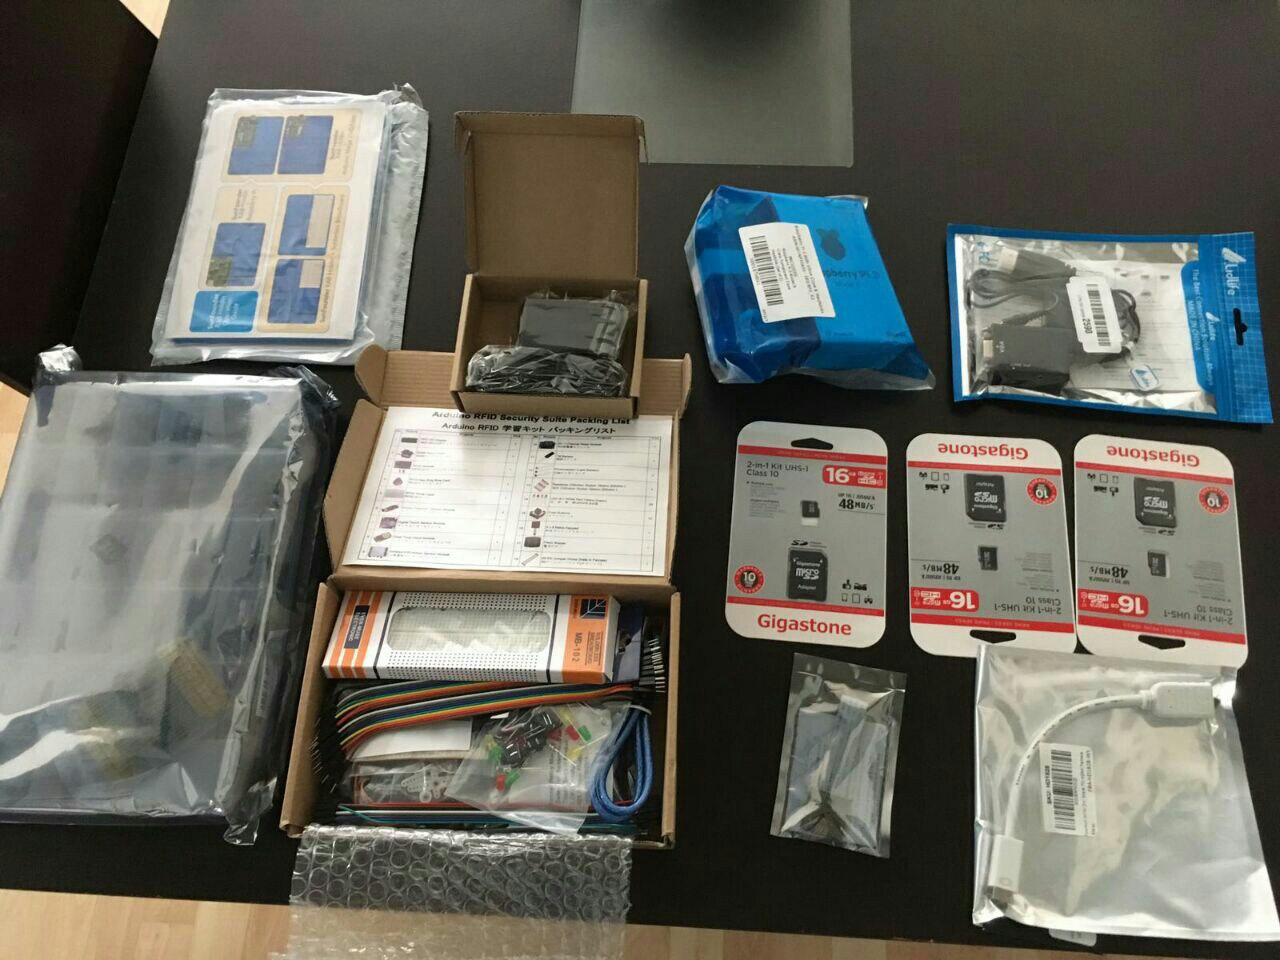
\includegraphics[scale=0.165]{./Figuras/sensores_recibidos.jpg}
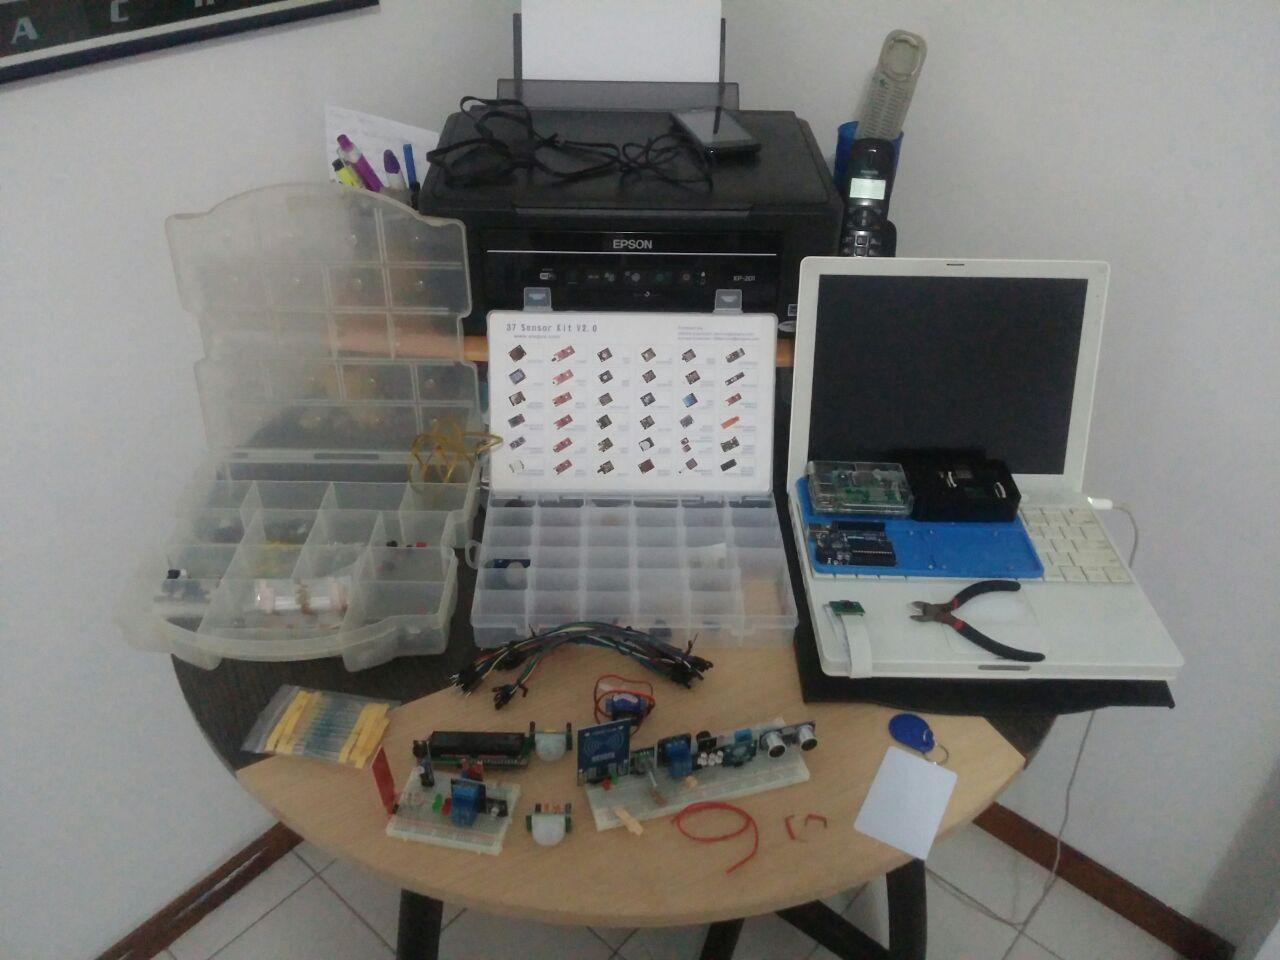
\includegraphics[scale=0.22]{./Figuras/sensores.jpg}
\caption{Elementos para prototipado de dispositivos}
\label{fig:sensores_recibido11s}
\vspace*{-10pt}
\end{figure}

Una vez organizados, se construyó uno a uno cada prototipo de dispositivo, comenzando por el prototipo de dispositivo para exteriores. Tomado el Arduino Uno y los sensores conectados a el, junto con la computadora iBook G4 como interfaz de despliegue del código a la placa programable y para captura y envío de los datos se procedió a desarrollar dos scripts:
\begin{itemize}
\item Un primer script en el lenguaje de programación Arduino con los drivers y la lógica de control de la placa programable  para los sensores y actuadores que fueron tomados según el diseño convenido anteriormente (figuras \ref{fig:arduino_ext} y \ref{fig:sensores_ext}).
\begin{figure}[!htb]
\centering
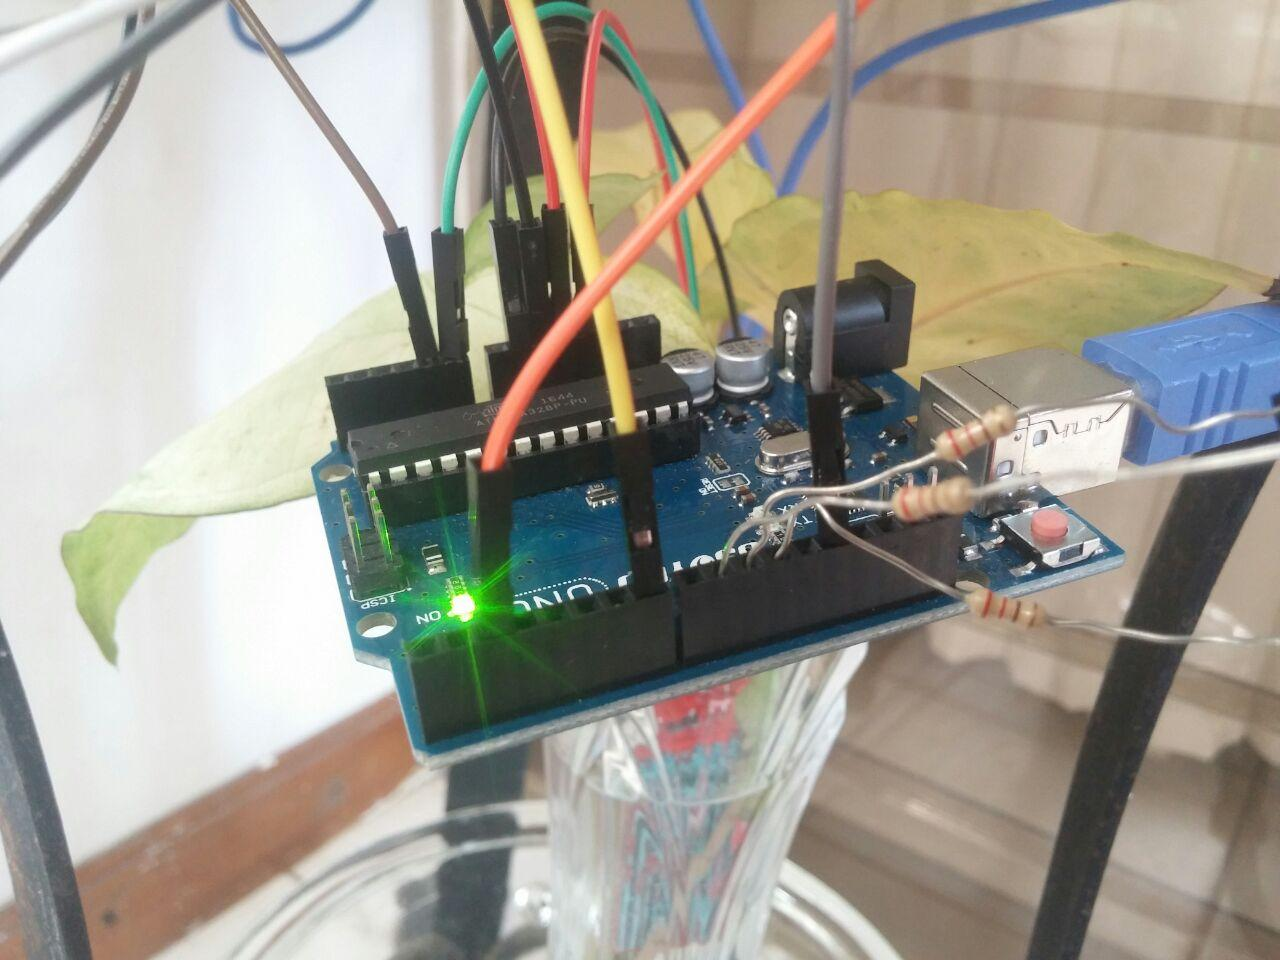
\includegraphics[scale=0.225]{./Figuras/arduino_ext.jpg}
\caption{Arduino Uno conectado a sensores y al iBook G4}
\label{fig:arduino_ext}
\end{figure}

\begin{figure}[!htb]
\centering
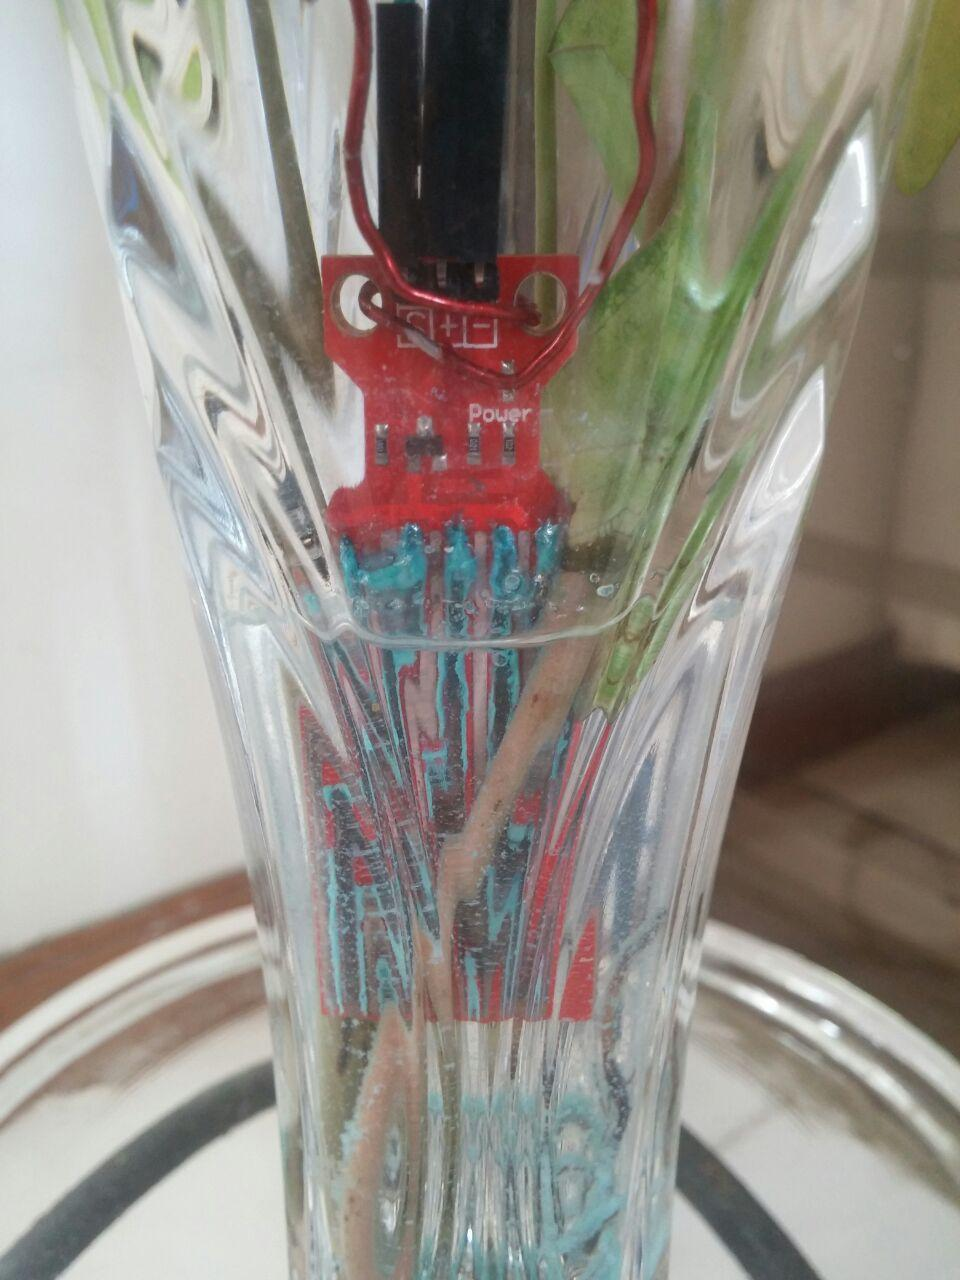
\includegraphics[scale=0.11]{./Figuras/sensor_agua.jpg}
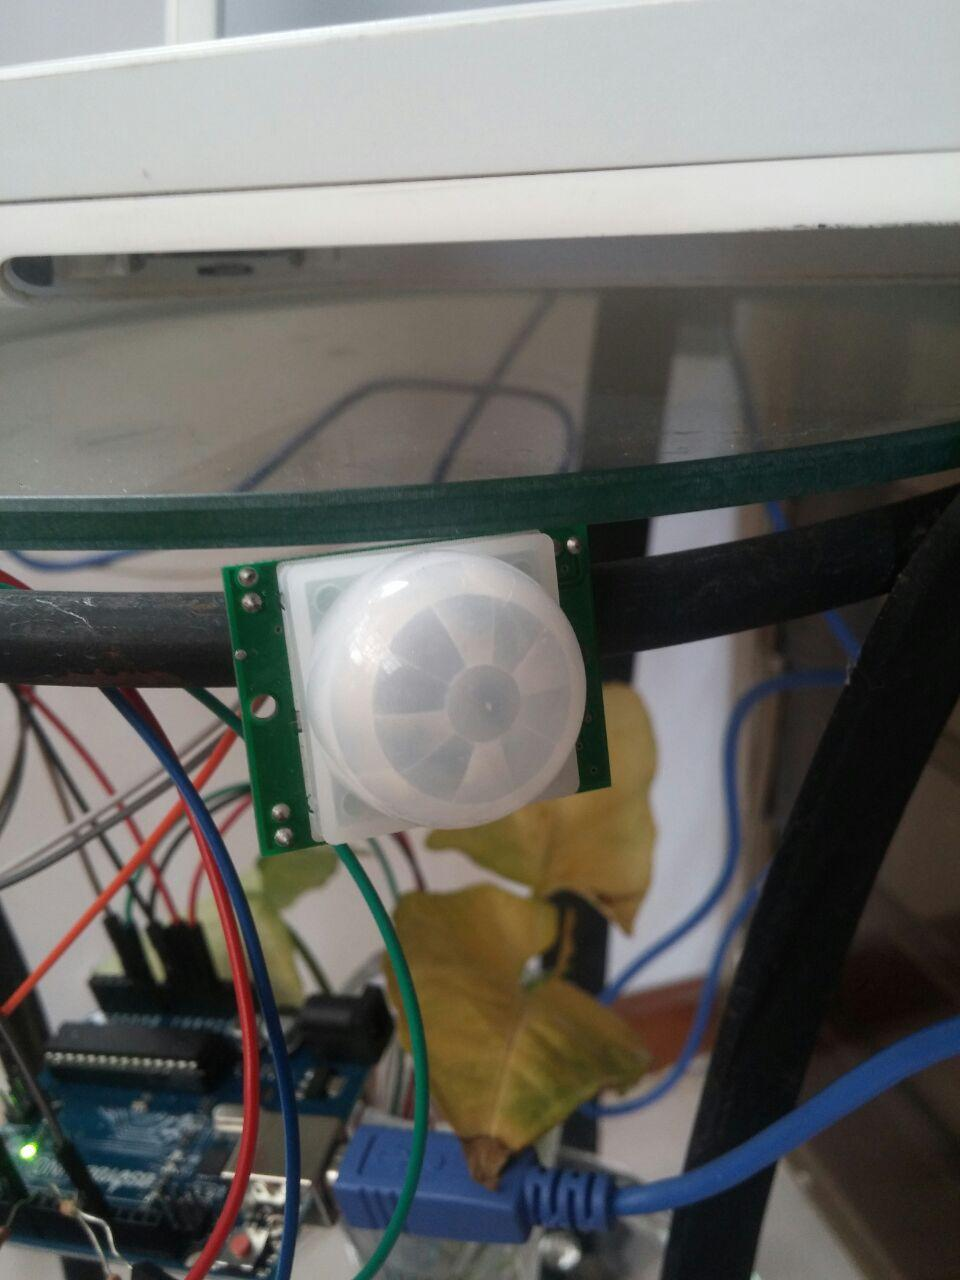
\includegraphics[scale=0.11]{./Figuras/pir_ext.jpg}
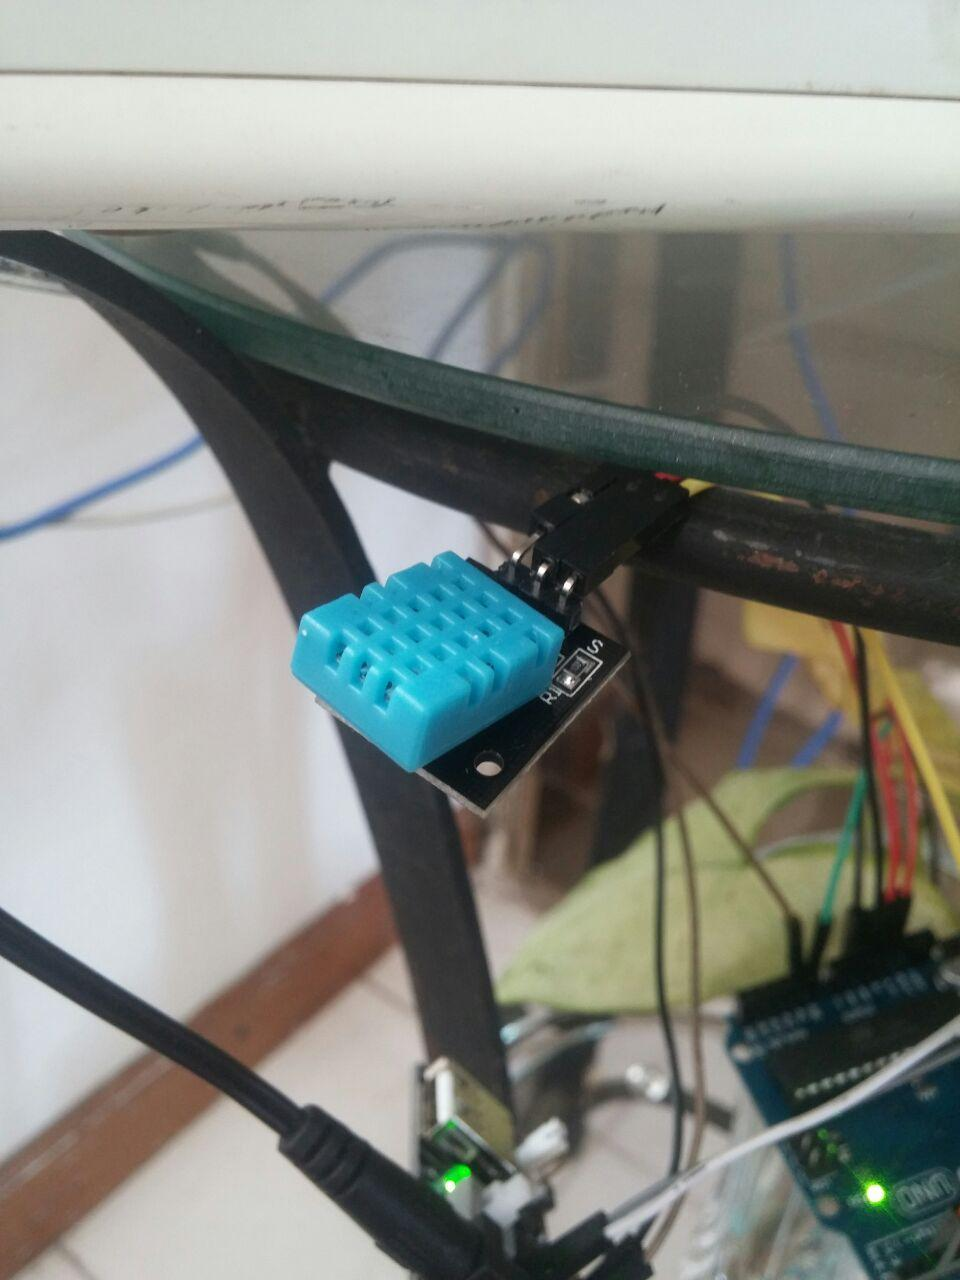
\includegraphics[scale=0.11]{./Figuras/temp_ext.jpg}
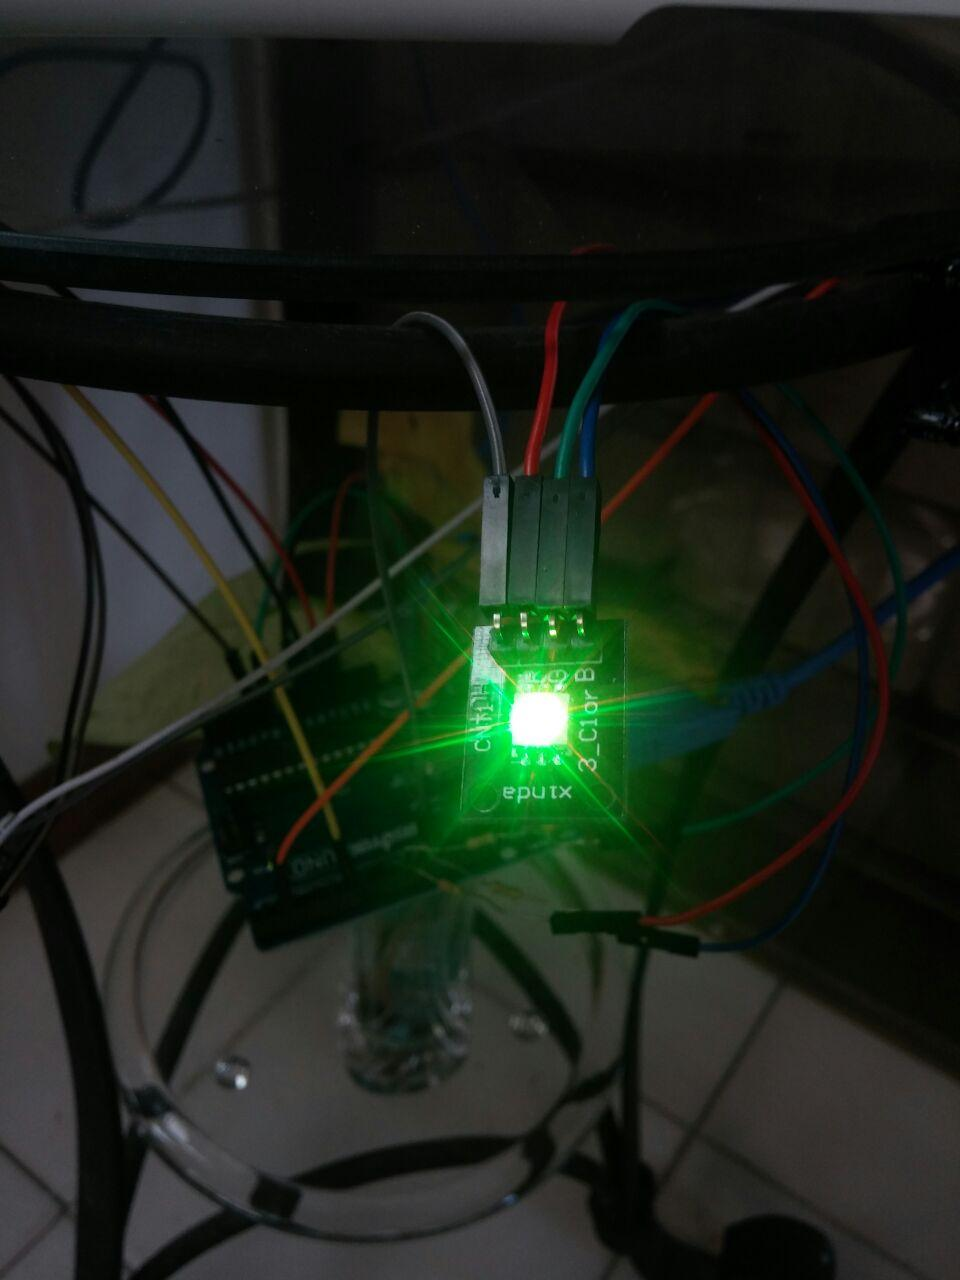
\includegraphics[scale=0.11]{./Figuras/rgb_ext.jpg}
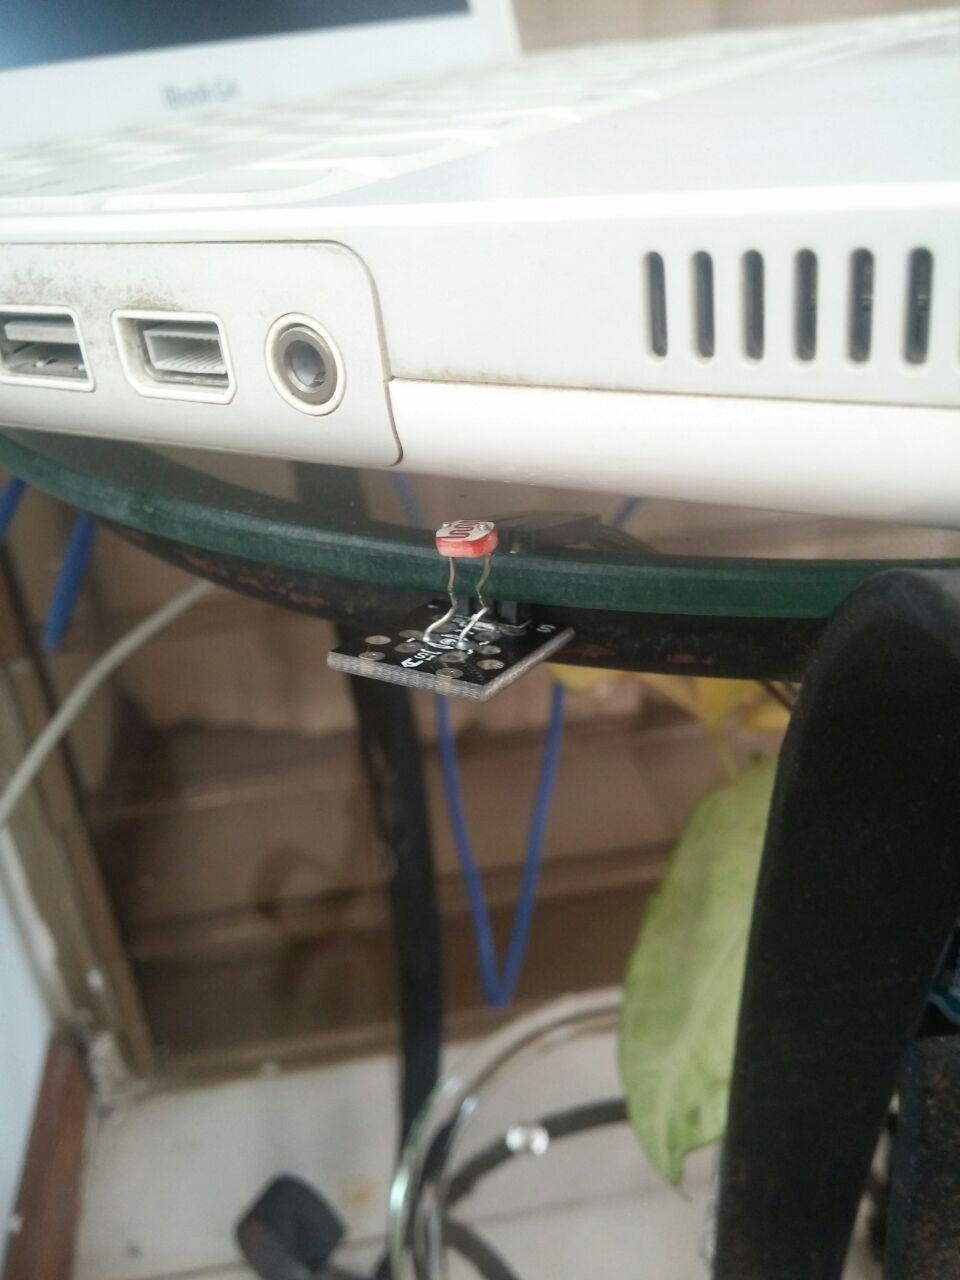
\includegraphics[scale=0.11]{./Figuras/fotorresistencia.jpg}
\caption{Sensores y actuadores en el exterior}
\label{fig:sensores_ext}
\vspace*{-10pt}
\end{figure}

\item Un segundo script en el lenguaje de programación Python con la capacidad de leer los datos seriales provenientes del Arduino Uno y con la capacidad de enviarlos a través del protocolo MQTT al broker %(véase figura \ref{fig:ibook_data}).
%\begin{figure}[htb]
%\centering
%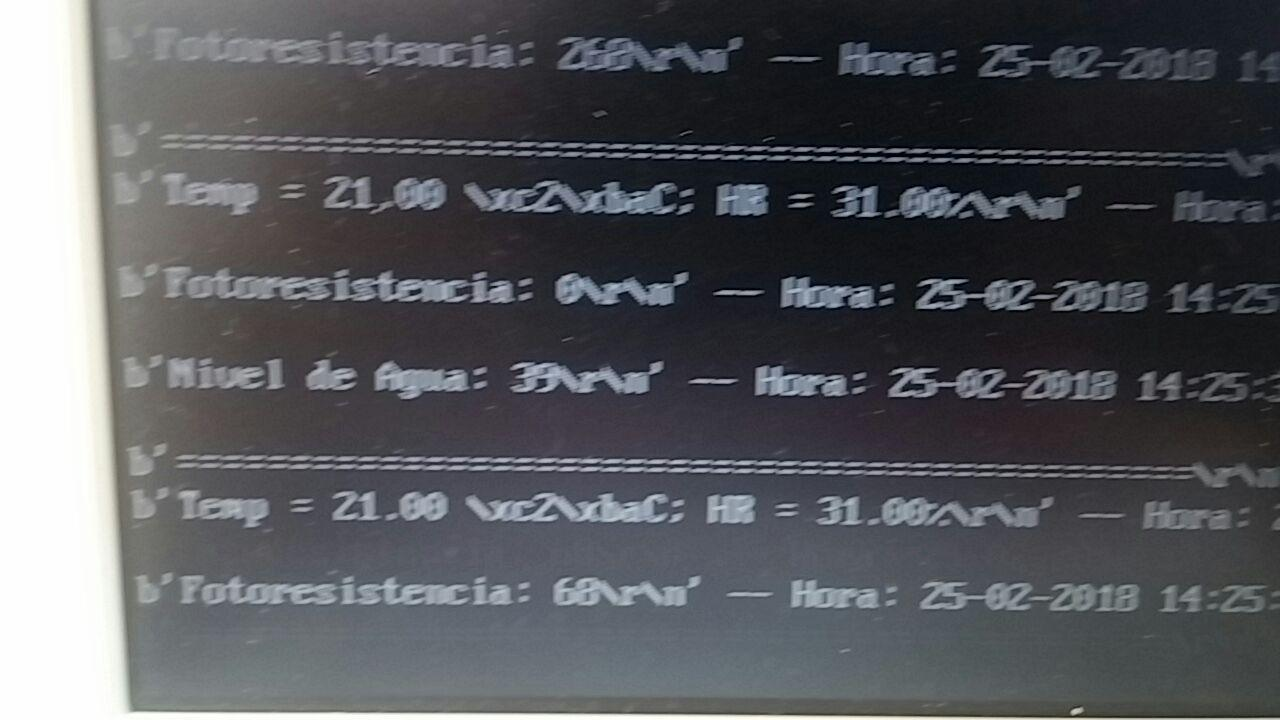
\includegraphics[scale=0.3]{./Figuras/ibook_data.jpg}
%\caption{Datos siendo capturados en el Ibook G4}
%\label{fig:ibook_data}
%\vspace*{-10pt}
%\end{figure}

\end{itemize}
Finalmente el dispositivo y el computador fueron colocados geográficamente en el balcón del apartamento para simular con la mayor precisión posible un ambiente exterior propiamente dicho.\\

El siguiente paso de manera similar consistió en construir el prototipo funcional del dispositivo IoT para ser interior del hogar. El dispositivo elegido para esta tarea fue uno de los dos Raspberry Pi 3 modelo B disponibles, así como la lista de sensores asociados para completar la tarea. De esta forma se ejecutaron las siguientes labores:
\begin{itemize}
\item Colocación de todos los sensores en un protoboard y de allí fue conectados al Raspberry Pi.

\item Instalación del sistema operativo Raspbian al dispositivo y se dejó preparado para utilizar una configuración headless, es decir, sin uso de monitor, solo acceso remoto.

\item Scripts en el lenguaje de programación Python por cada sensor y actuador utilizado. 

\item Construcción de una carcasa alrededor del dispositivo y el protoboard con la ayuda de bloques de lego como se puede observar en la figura \ref{fig:rpi3javier_indoor}. Su disposición final geográficamente fue situado en el centro del apartamento.
\begin{figure}[!htb]
\centering
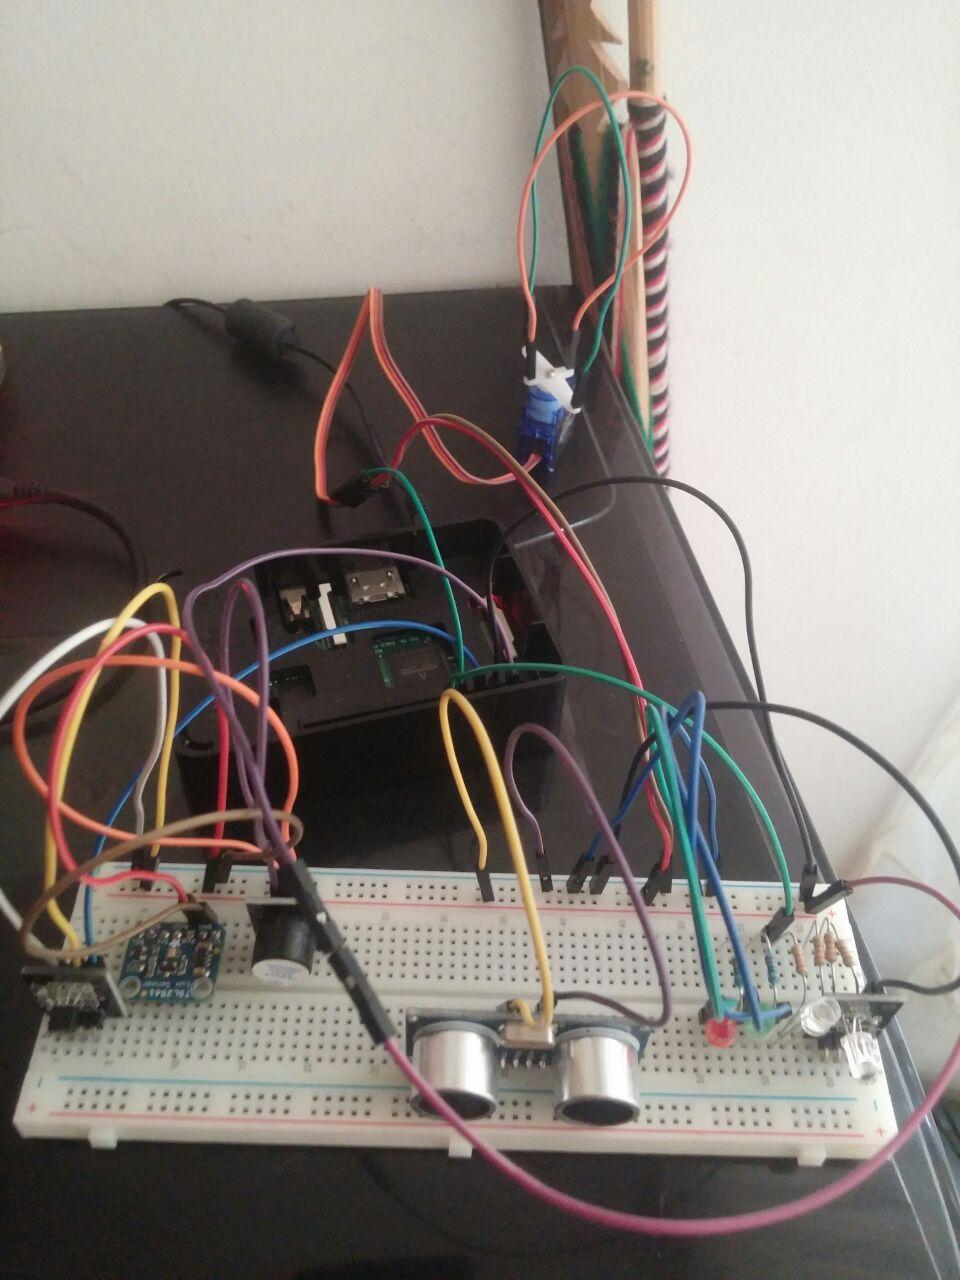
\includegraphics[scale=0.165]{./Figuras/rpi3javier_proto.jpg}
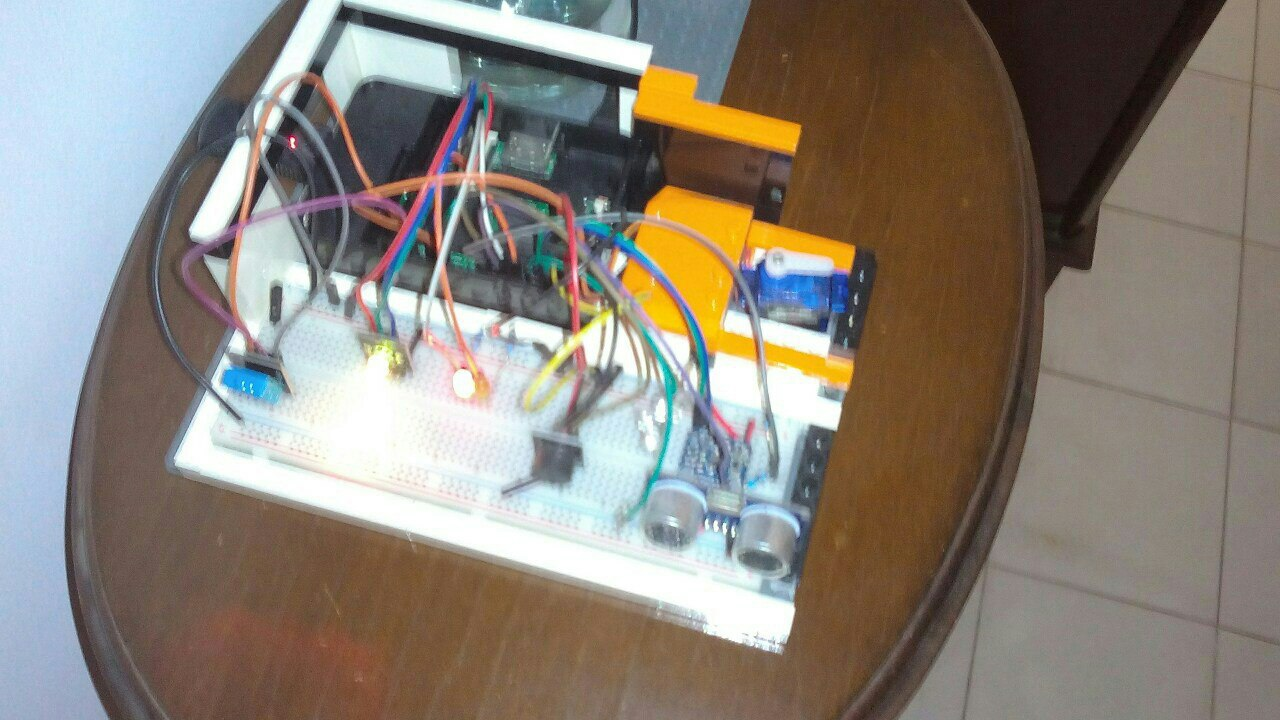
\includegraphics[scale=0.22]{./Figuras/rpi3javier_final.jpg}
\caption{Sensor IoT en el interior del hogar antes y despues de su validación}
\label{fig:rpi3javier_indoor}
\vspace*{-10pt}
\end{figure}
\end{itemize} 

Luego, se continuó con los dos prototipos que representan elementos de seguridad. Para ellos se utilizaron el Raspberry Pi Zero y el Raspberry Pi 3 modelo B restante. Para poder dejar activos los elementos correspondientes a ellos se siguieron los siguientes pasos:
\begin{itemize}
\item  Colocación de todos los sensores y actuadores en un protoboard y al  Raspberry Pi Zero.

\item Instalación del sistema operativo Raspbian al dispositivo y se dejó preparado para utilizar una configuración headless, es decir, sin uso de monitor, solo acceso remoto.

\item Conexión directa del Raspberry Pi Zero al Raspberry Pi 3 modelo B para proveer de conectividad a la red al dispositivo. 

\item Desarrollo de scripts en el lenguaje de programación Python por cada sensor y actuador utilizado en Raspberry Pi zero.

\item Desarrollo de un modelo de inteligencia artificial en el lenguaje de programación Python para usar la cámara acoplada al Raspberry Pi 3 modelo B de forma que reconociera las caras de los habitantes que entrasen al hogar.  

\item Se instalaron los elementos necesarios para dar futuro soporte al despliegue de la aplicación web HAMACA en el Raspberry Pi 3 modelo B, así como también se creó un punto de acceso para los dispositivos se pudieran conectar a el de manera independiente de la red del hogar. 
\end{itemize}

Al finalizar el desarrollo del prototipo de dispositivo este fue situado validado y colocado en la entrada del hogar (figura \ref{fig:rpi3peter_zero}), cuestión que fuera centro neuralgico de los sensores de seguridad. Aparte la capacidad de cómputo del Raspberry Pi 3 modelo B también estaría a disposición siendo el elemento de cómputo definido para la siguiente etapa de la implementación.
\begin{figure}[!htb]
\centering
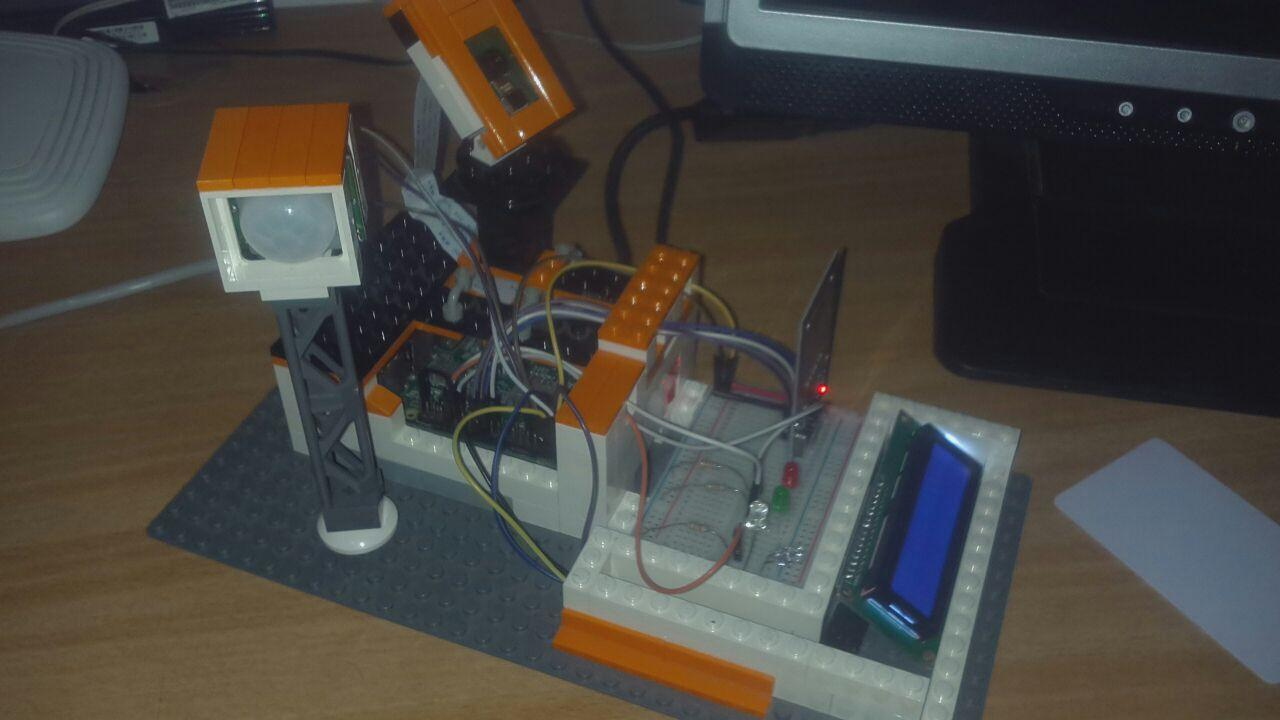
\includegraphics[scale=0.22]{./Figuras/rpi3peter_zero_proto.jpg}
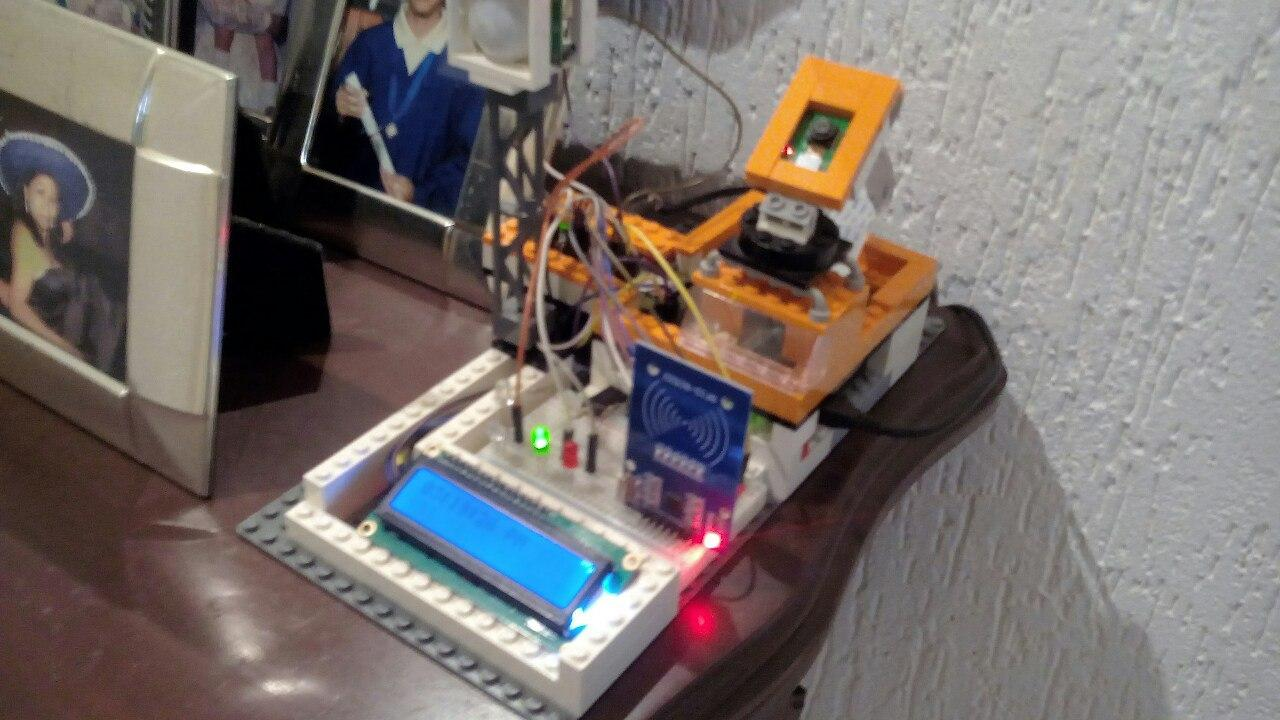
\includegraphics[scale=0.17]{./Figuras/rpi3peter_zero.jpg}
\caption{Sensor IoT en el interior del hogar antes y después de su validación}
\label{fig:rpi3peter_zero}
\vspace*{-10pt}
\end{figure}


\subsection{Implementación de la Aplicación Web HAMACA}
Por el lado de la aplicación web HAMACA, el proceso de implementación fue llevado a cabo siguiendo los lineamientos de las metodologías ágiles, con entregables incrementales, rápidas iteraciones con nuevas características y corrección de errores. Se estimó inicialmente un período de desarrollo de aproximadamente un mes y medio para tener todos los aspectos necesarios para cubrir los objetivos planteados y dar una propuesta de solución al problema de investigación.\\

Los pasos que se siguieron para poder desarrollar y desplegar la aplicación web fueron los siguientes:

\subsubsection{Infraestructura}
Por el lado de la infraestructura, al tener como elemento de cómputo para despliegue un Raspberry Pi 3 Modelo B, el sistema operativo base utilizado fue raspbian, un flavor de Debian, una opción popular y fácil de utilizar para los desarrollos de software.\\

Directamente sobre el sistema operativo se instalaron todos y cada uno de los paquetes, base de datos (InfluxDB y PostgreSQL), herramientas a integrar (Grafana y Node-Red), la implementación de MQTT, así como también el ambiente de Python 3 para manejar la webapp.  Este proceso cambió para luego dejar la mayor cantidad de elementos posibles para ser utilizados bajo el esquema de contenedores docker, siendo migrados a esa forma la base de datos InfluxDB, y las herramientas Grafana y Node-Red. Lo cual permite un despliegue mucho más rápido en cualquier ambiente nuevo, así como modularizar el proyecto de una mejor forma.

\subsubsection{Configuración de Entorno}
Una vez instalados los diversos paquetes y herramientas se procedió con la configuración de todos los elementos previos a la parte de desarrollo.
\begin{itemize}
\item La configuración asociada a la comunicación entre los dispositivos basados en el broker MQTT instalado. 
\item La creación de una base de datos en InfluxDB, junto con un usuario y métodos de acceso de forma de almacenar a través del backend de la aplicación toda la data relativa a los dispositivos. 
\item Despliegue de la herramienta de visualización y monitoreo Grafana. Configuraciones asociadas para la conexión a la fuente de datos (base de datos InfluxDB) así como también el acceso y privilegios de gestión de cuadros de mando sin la necesidad de un usuario logeado y con privilegios asociados.
\item Despliegue de la herramienta Node-Red para el control de dispositivos. Se le armó configuraciones para poder crear interfaces basadas en cuadros de mando para poder realizar tareas de control sobre sensores y actuadores de los dispositivos. También se probaron y validaron la posibilidad de generar flujos de tareas para los dispositivos a través de esta herramienta.
\end{itemize}

\subsubsection{Desarrollo de la Aplicación Web HAMACA}
Finalmente con el entorno configurado se procedió con el desarrollo de la aplicación web HAMACA. Fue diseñada como una aplicación web liviana y sencilla haciendo uso del framework de desarrollo Django para el lenguaje de programación Pyhon en su versión 3.\\

Al comenzar el proyecto se creó la aplicación a partir de la plantilla de instrucciones que provee el framework, junto con la definición de utilizar PostgreSQL como base datos, puesto que es una respuesta más robusta que SQLite (base de datos por defecto) tanto para el soporte mismo de la aplicación como de sus futuros procesos. Es así como luego de configurada la base y siguiendo las instrucciones se generó en la base de datos de HAMACA los modelos que podemos observar en la figura \ref{fig:django_schema}.
\begin{figure}[!htb]
\centering
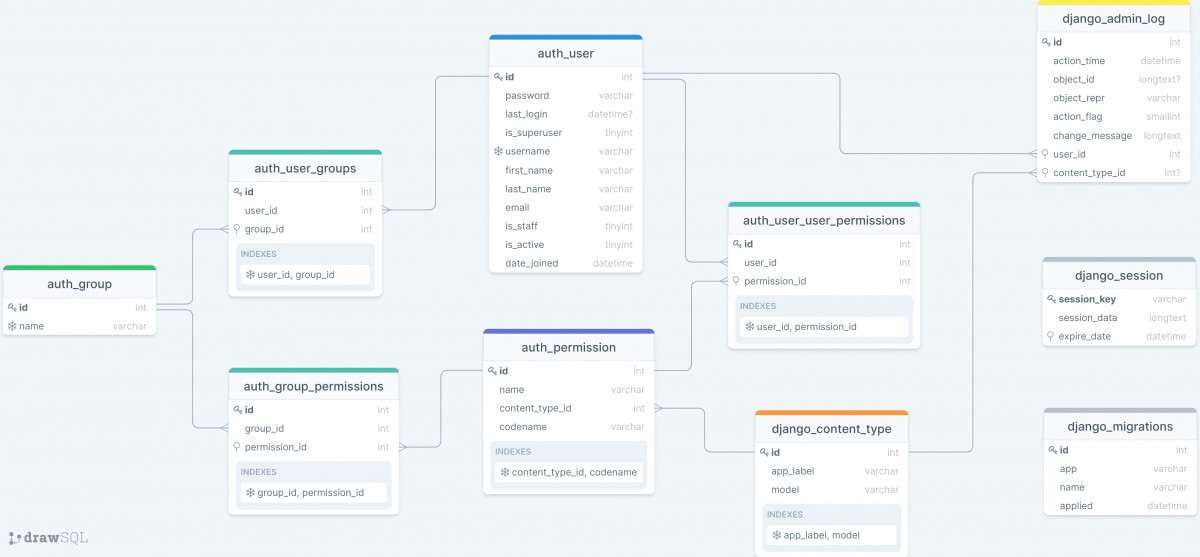
\includegraphics[scale=0.505]{./Figuras/django_schema.jpg}
\caption{Modelo autogenerado por el framework Django}
\label{fig:django_schema}
%\vspace*{-5pt}
\end{figure}

En el argot de Django, este primer paso se le llama migración. Con ello se comienzo con el desarrollo del primer modulo de control y acceso a la aplicación basado en los aspectos de roles y privilegios del que se dispone en el framework.\\

Es en este punto donde también se estructuran las bases para un desarrollo modular en el que se fueron integrando progresiva e incrimentalmente nuevos elementos entre los cuales se encuentran las librerías comunes, plantillas para los aspectos visuales, los elementos estáticos como las fuentes para los textos, gráficos y colores.\\ 

Se comenzó con un primer módulo desarrollado para el acceso a la aplicación 
%(figura \ref{fig:login_ui}) 
junto con las de configuraciones (figura \ref{fig:hamaca_config}), el cual contiene las herramientas de gestión de la aplicación, como la administración de usuarios, así como la capacidad de cambar la ubicación de las herramientas integradas, sea que se encuentren de manera local o en algún lugar que pueda ser accedido por este desarrollo.\\
%\begin{figure}[!htb]
%\centering
%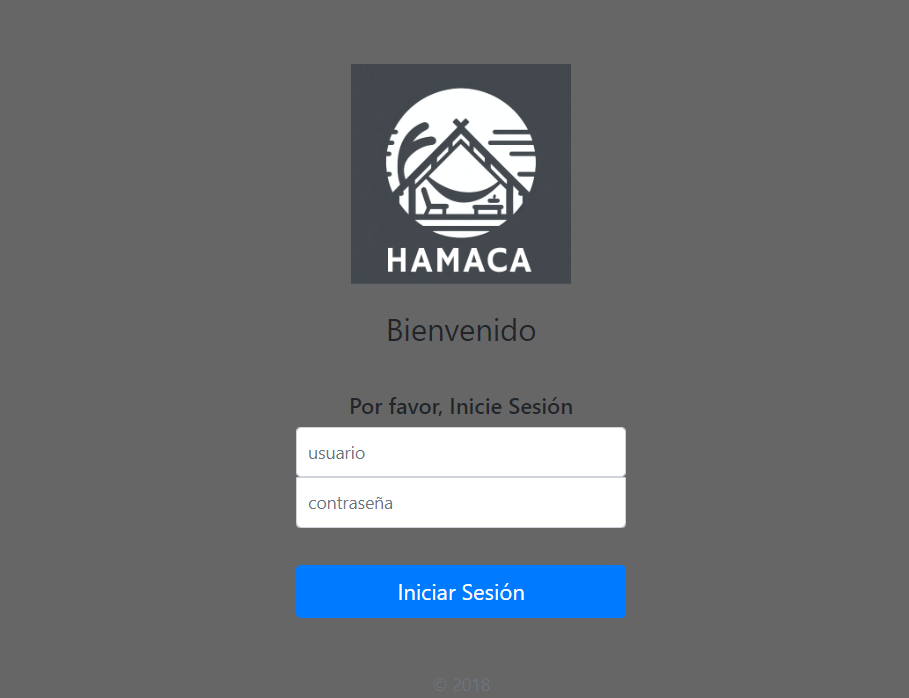
\includegraphics[scale=0.2]{./Figuras/login_ui.png}
%\caption{Interfaz de inicio de sesión para los usuarios}
%\label{fig:login_ui}
%\vspace*{-10pt}
%\end{figure}

\begin{figure}[htb]
\centering
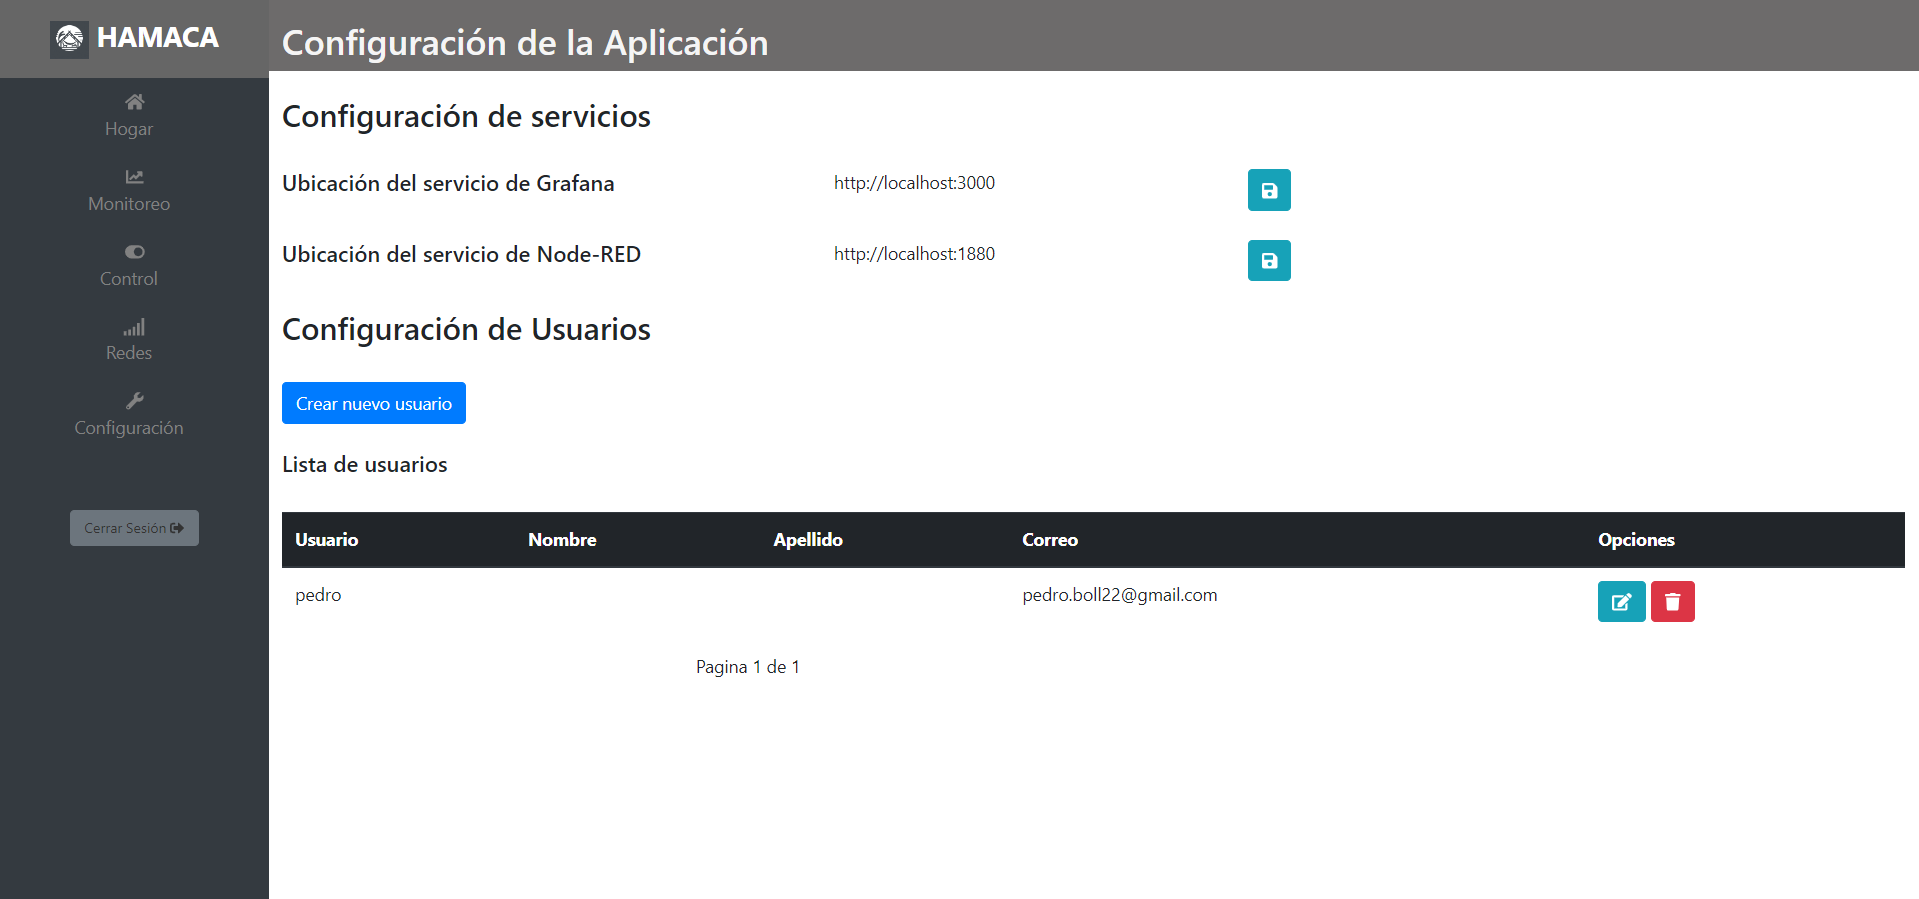
\includegraphics[scale=0.2]{./Figuras/hamaca_config.png}
\caption{Interfaz de configuración de la aplicación}
\label{fig:hamaca_config}
\vspace*{-10pt}
\end{figure}

A partir del punto anterior se creó un modulo de Monitoreo el cual contiene la lógica para integrar de manera adecuada la herramienta Grafana para visualización y monitoreo de datos, de forma que los usuarios puedan crear sus cuadros de mando de una manera sencilla y directa.\\ %(figura \ref{fig:hamaca_grafana}).\\

%\begin{figure}[!htb]
%\centering
%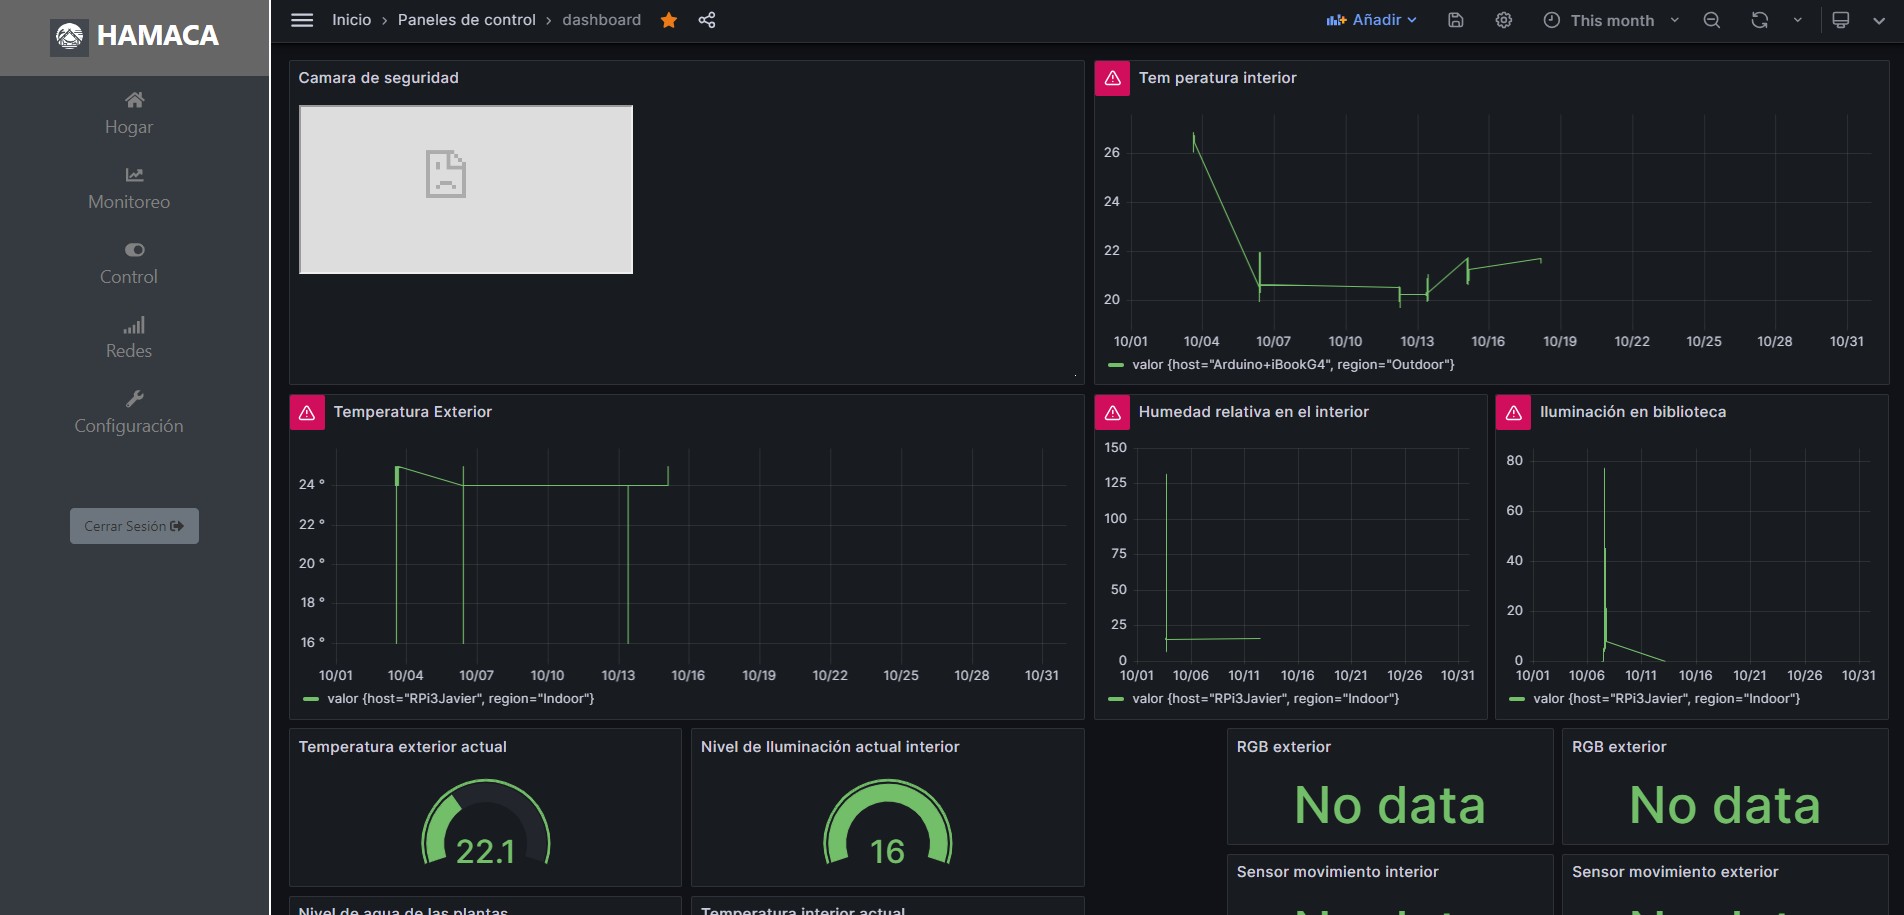
\includegraphics[scale=0.23]{./Figuras/hamaca_grafana.png}
%\caption{Interfaz de visualización de datos con la herramienta Grafana embebida}
%\label{fig:hamaca_grafana}
%\vspace*{-10pt}
%\end{figure}

De manera análoga se creó un modulo de control y un home que contienen la lógica de la integración de la herramienta Node-Red para llevar a cabo las labores de controlar y gestionar flujos de trabajo complejos con los dispositivos.\\
%(figura \ref{fig:hamaca_nodered}).\\ 

%\begin{figure}[!htb]
%\centering
%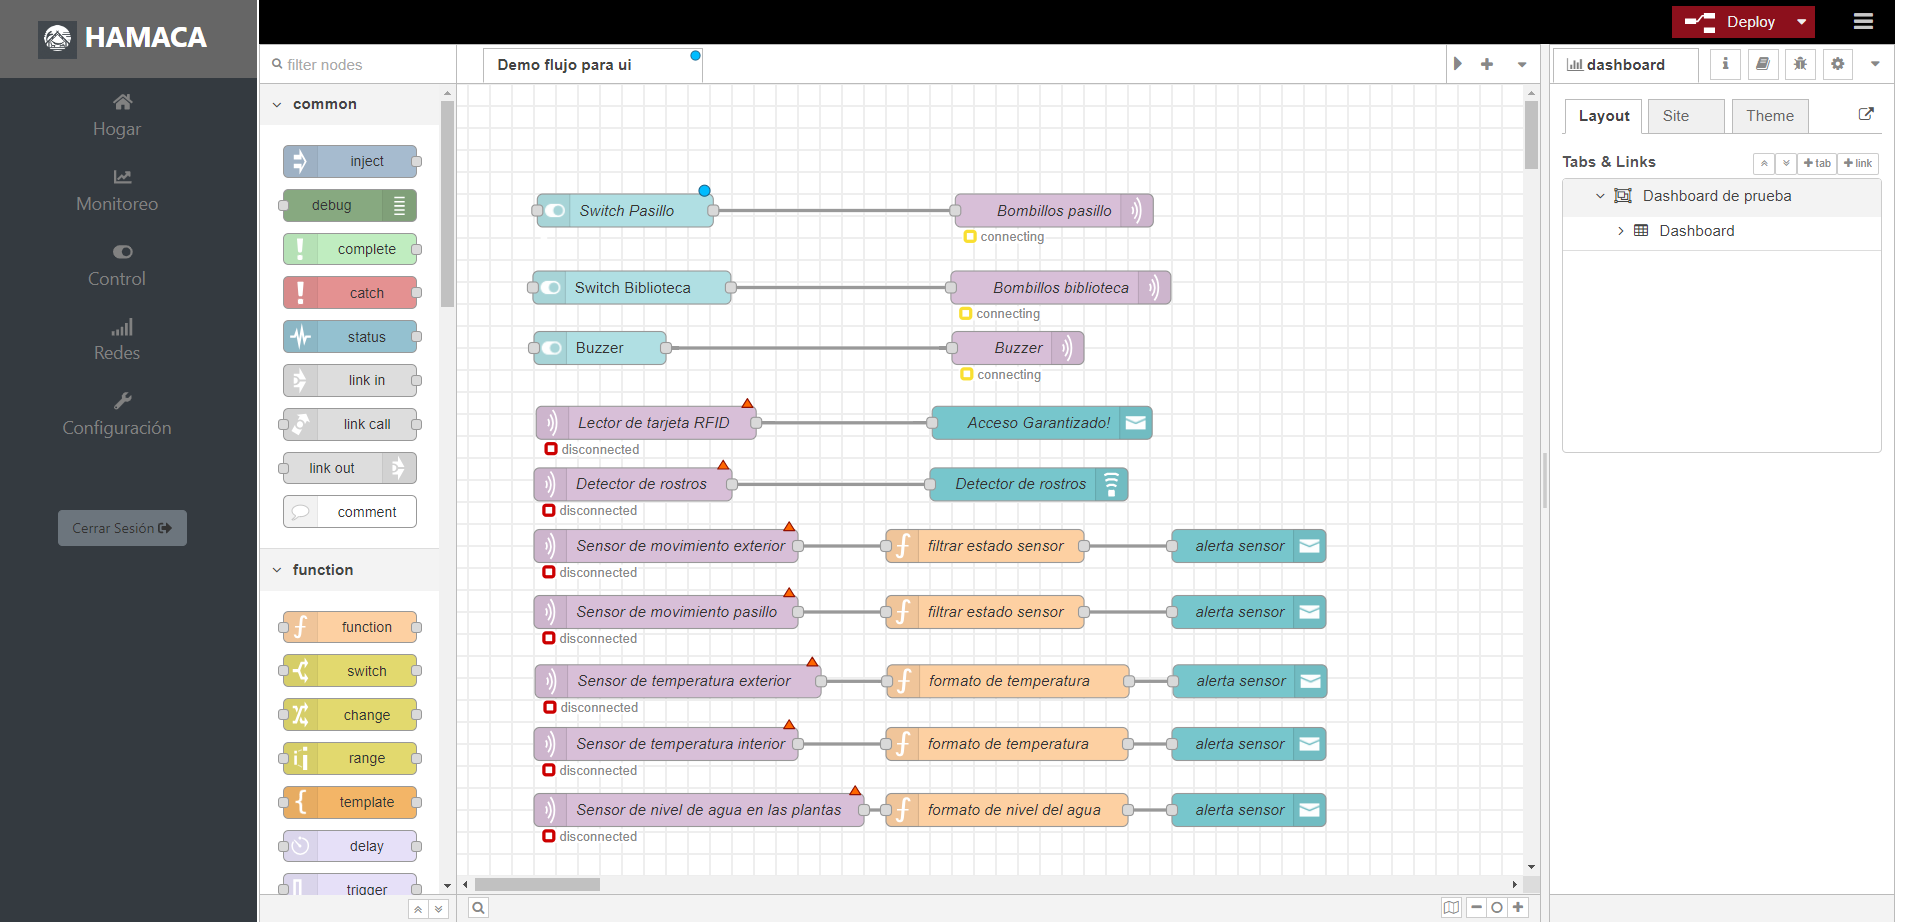
\includegraphics[scale=0.21]{./Figuras/hamaca_nodered.png}
%\caption{Interfaz de flujos de automatización con la herramienta Node-Red embebida}
%\label{fig:hamaca_nodered}
%\vspace*{-10pt}
%\end{figure}

El home de la aplicación particularmente se convierte en un punto donde se muestran los cuadros de mando creados para manipular (e incluso observar) sensores y actuadores de aquellos dispositivos que registremos en los flujos para mostrar. Por último pero no menos importante se creó un apartado de redes en el cual se pueden observar los registros de las comunicaciones realizadas entre los dispositivos y el broker, así como otras métricas asociadas a ello (figura  \ref{fig:hamaca_redes}).\\

%\begin{figure}[!htb]
%\centering
%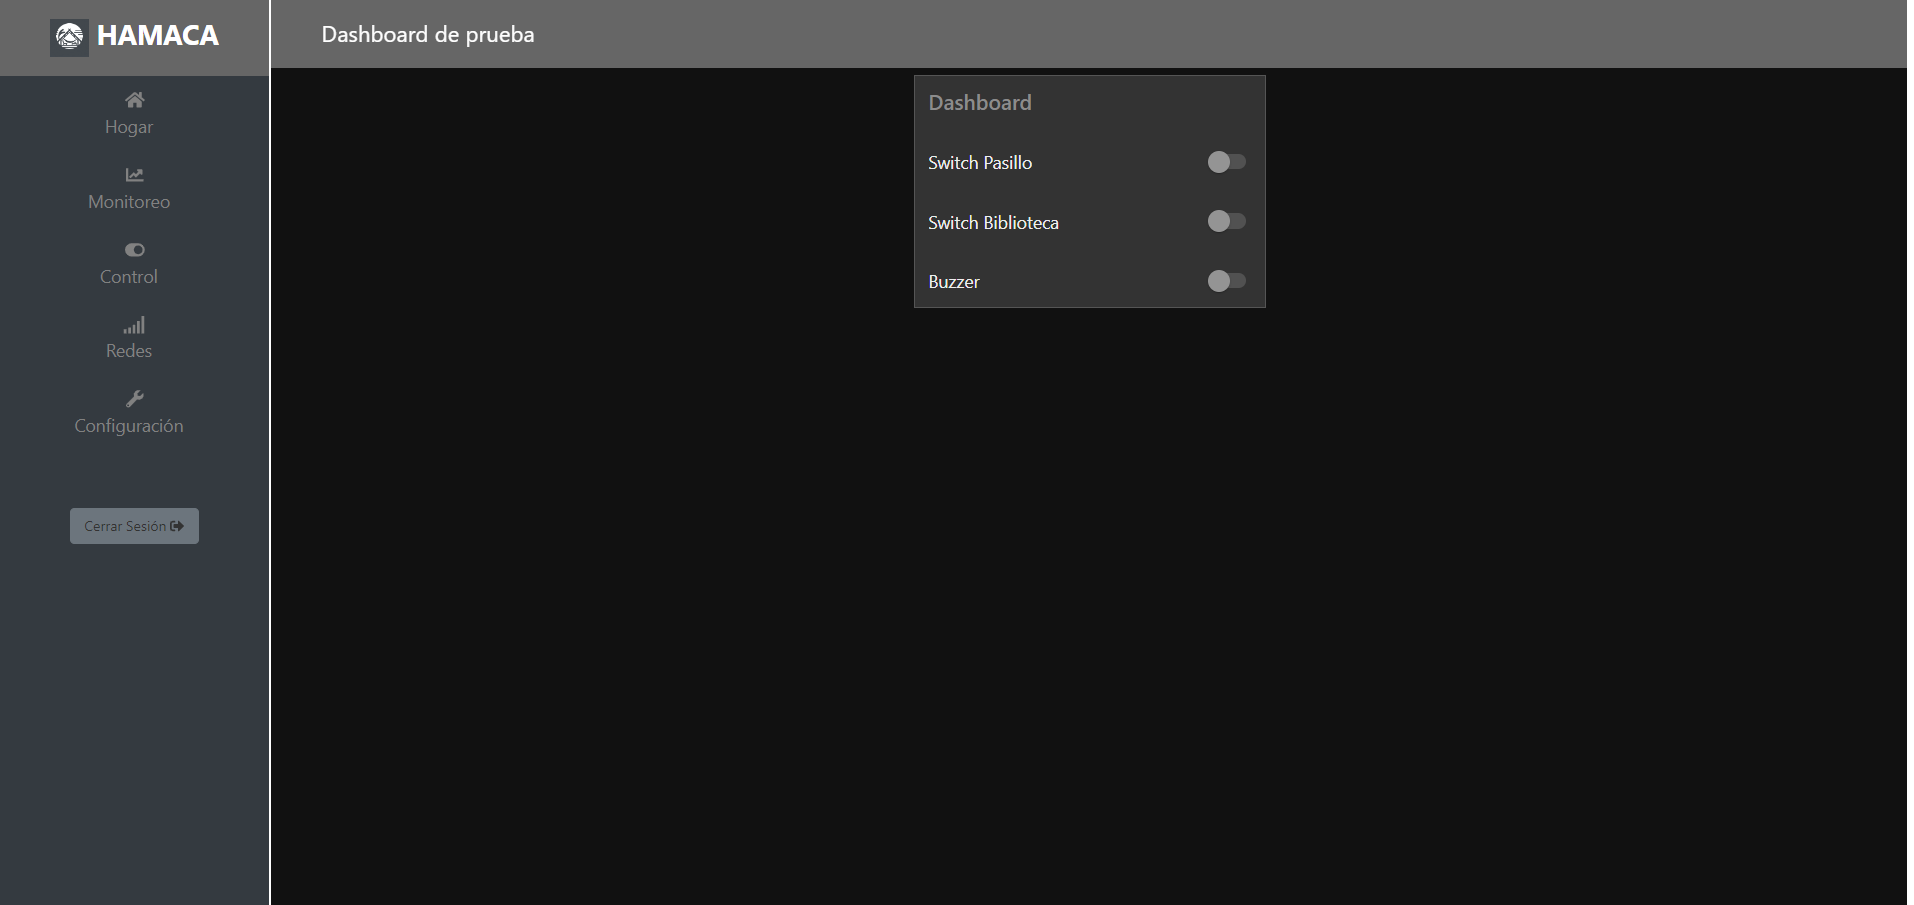
\includegraphics[scale=0.2]{./Figuras/hamaca_home.png}
%\caption{Interfaz de control de dispositivos a través del dashboard de Node-Red}
%\label{fig:hamaca_home}
%\vspace*{-10pt}
%\end{figure}

\begin{figure}[!htb]
\centering
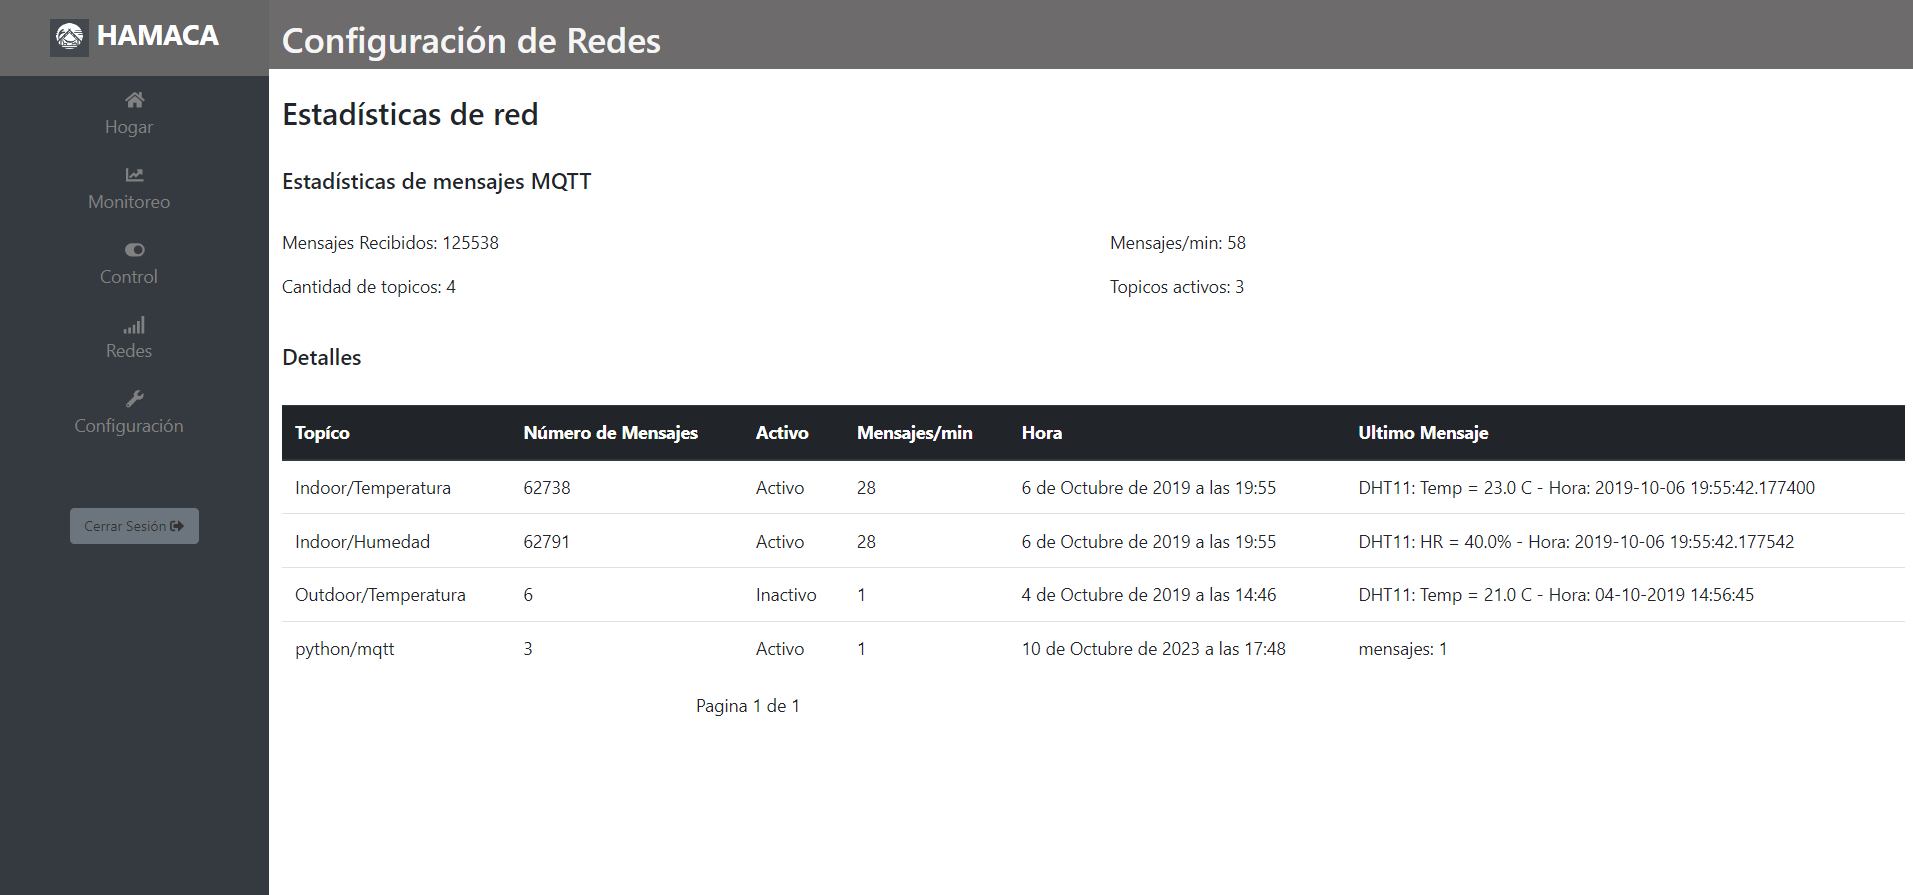
\includegraphics[scale=0.2]{./Figuras/hamaca_redes.png}
\caption{Interfaz de la aplicación para la configuración y visualización de métricas de red}
\label{fig:hamaca_redes}
\vspace*{-10pt}
\end{figure}

Luego del desarrollo de cada modulo y aunque no todos los módulos interactuan con la base de datos se realizó nuevamente el proceso de migración, de forma que la base de datos se adaptara a los requerimientos nuevos de los módulos existentes. Así la base de datos se le agregaron dos nuevas tablas como se pueden observar en la figura \ref{fig:psql_hamaca_db}
\begin{figure}[!htb]
\centering
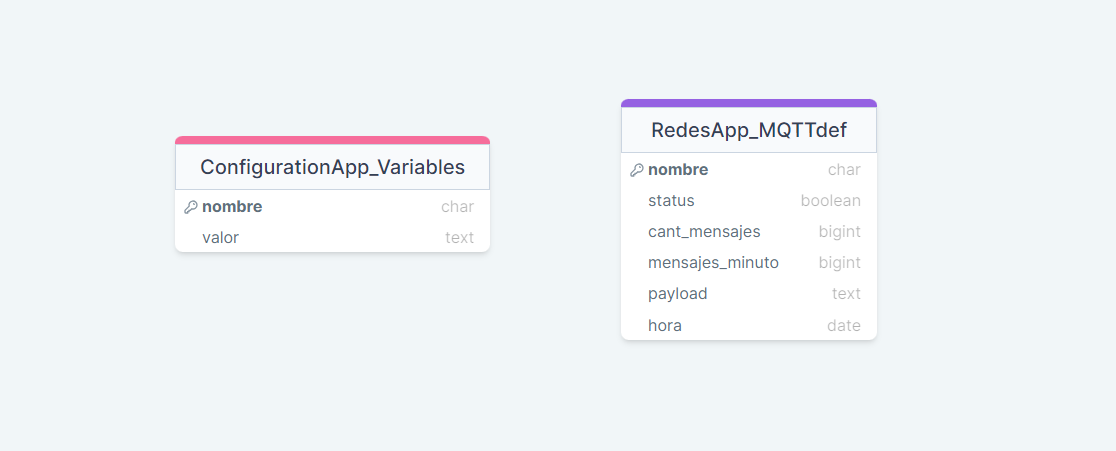
\includegraphics[scale=0.35]{./Figuras/psql_hamaca_db.png}
\caption{Modelo de la base de datos HAMACA}
\label{fig:psql_hamaca_db}
\vspace*{-10pt}
\end{figure}
